\documentclass{tufte-book}

\hypersetup{colorlinks}% uncomment this line if you prefer colored hyperlinks (e.g., for onscreen viewing)

%%
% Book metadata
\title{Daily Problem Sets Vol. I}
\author[Alex Cooper]{Alex Cooper}
\publisher{adrcooper.com}

%%
% If they're installed, use Bergamo and Chantilly from www.fontsite.com.
% They're clones of Bembo and Gill Sans, respectively.
\IfFileExists{bergamo.sty}{\usepackage[osf]{bergamo}}{}% Bembo
\IfFileExists{chantill.sty}{\usepackage{chantill}}{}% Gill Sans

\usepackage{microtype}

%%
% For nicely typeset tabular material
\usepackage{booktabs}

%%
% For graphics / images
\usepackage{graphicx}
\setkeys{Gin}{width=\linewidth,totalheight=\textheight,keepaspectratio}
\graphicspath{{graphics/}}

\usepackage{array}
\providecommand{\tabularnewline}{\\}

% The fancyvrb package lets us customize the formatting of verbatim
% environments.  We use a slightly smaller font.
\usepackage{fancyvrb}
\fvset{fontsize=\normalsize}

%%
% Prints argument within hanging parentheses (i.e., parentheses that take
% up no horizontal space).  Useful in tabular environments.
\newcommand{\hangp}[1]{\makebox[0pt][r]{(}#1\makebox[0pt][l]{)}}

%%
% Prints an asterisk that takes up no horizontal space.
% Useful in tabular environments.
\newcommand{\hangstar}{\makebox[0pt][l]{*}}

%%
% Prints a trailing space in a smart way.
\usepackage{xspace}

%%
% Some shortcuts for Tufte's book titles.  The lowercase commands will
% produce the initials of the book title in italics.  The all-caps commands
% will print out the full title of the book in italics.
\newcommand{\vdqi}{\textit{VDQI}\xspace}
\newcommand{\ei}{\textit{EI}\xspace}
\newcommand{\ve}{\textit{VE}\xspace}
\newcommand{\be}{\textit{BE}\xspace}
\newcommand{\VDQI}{\textit{The Visual Display of Quantitative Information}\xspace}
\newcommand{\EI}{\textit{Envisioning Information}\xspace}
\newcommand{\VE}{\textit{Visual Explanations}\xspace}
\newcommand{\BE}{\textit{Beautiful Evidence}\xspace}

\newcommand{\TL}{Tufte-\LaTeX\xspace}

% Prints the month name (e.g., January) and the year (e.g., 2008)
\newcommand{\monthyear}{%
  \ifcase\month\or January\or February\or March\or April\or May\or June\or
  July\or August\or September\or October\or November\or
  December\fi\space\number\year
}


% Prints an epigraph and speaker in sans serif, all-caps type.
\newcommand{\openepigraph}[2]{%
  %\sffamily\fontsize{14}{16}\selectfont
  \begin{fullwidth}
  \sffamily\large
  \begin{doublespace}
  \noindent\allcaps{#1}\\% epigraph
  \noindent\allcaps{#2}% author
  \end{doublespace}
  \end{fullwidth}
}

% Inserts a blank page
\newcommand{\blankpage}{\newpage\hbox{}\thispagestyle{empty}\newpage}

\usepackage{units}

% Typesets the font size, leading, and measure in the form of 10/12x26 pc.
\newcommand{\measure}[3]{#1/#2$\times$\unit[#3]{pc}}

% Macros for typesetting the documentation
\newcommand{\hlred}[1]{\textcolor{Maroon}{#1}}% prints in red
\newcommand{\hangleft}[1]{\makebox[0pt][r]{#1}}
\newcommand{\hairsp}{\hspace{1pt}}% hair space
\newcommand{\hquad}{\hskip0.5em\relax}% half quad space
\newcommand{\TODO}{\textcolor{red}{\bf TODO!}\xspace}
\newcommand{\ie}{\textit{i.\hairsp{}e.}\xspace}
\newcommand{\eg}{\textit{e.\hairsp{}g.}\xspace}
\newcommand{\na}{\quad--}% used in tables for N/A cells
\providecommand{\XeLaTeX}{X\lower.5ex\hbox{\kern-0.15em\reflectbox{E}}\kern-0.1em\LaTeX}
\newcommand{\tXeLaTeX}{\XeLaTeX\index{XeLaTeX@\protect\XeLaTeX}}
% \index{\texttt{\textbackslash xyz}@\hangleft{\texttt{\textbackslash}}\texttt{xyz}}
\newcommand{\tuftebs}{\symbol{'134}}% a backslash in tt type in OT1/T1
\newcommand{\doccmdnoindex}[2][]{\texttt{\tuftebs#2}}% command name -- adds backslash automatically (and doesn't add cmd to the index)
\newcommand{\doccmddef}[2][]{%
  \hlred{\texttt{\tuftebs#2}}\label{cmd:#2}%
  \ifthenelse{\isempty{#1}}%
    {% add the command to the index
      \index{#2 command@\protect\hangleft{\texttt{\tuftebs}}\texttt{#2}}% command name
    }%
    {% add the command and package to the index
      \index{#2 command@\protect\hangleft{\texttt{\tuftebs}}\texttt{#2} (\texttt{#1} package)}% command name
      \index{#1 package@\texttt{#1} package}\index{packages!#1@\texttt{#1}}% package name
    }%
}% command name -- adds backslash automatically
\newcommand{\doccmd}[2][]{%
  \texttt{\tuftebs#2}%
  \ifthenelse{\isempty{#1}}%
    {% add the command to the index
      \index{#2 command@\protect\hangleft{\texttt{\tuftebs}}\texttt{#2}}% command name
    }%
    {% add the command and package to the index
      \index{#2 command@\protect\hangleft{\texttt{\tuftebs}}\texttt{#2} (\texttt{#1} package)}% command name
      \index{#1 package@\texttt{#1} package}\index{packages!#1@\texttt{#1}}% package name
    }%
}% command name -- adds backslash automatically
\newcommand{\docopt}[1]{\ensuremath{\langle}\textrm{\textit{#1}}\ensuremath{\rangle}}% optional command argument
\newcommand{\docarg}[1]{\textrm{\textit{#1}}}% (required) command argument
\newenvironment{docspec}{\begin{quotation}\ttfamily\parskip0pt\parindent0pt\ignorespaces}{\end{quotation}}% command specification environment
\newcommand{\docenv}[1]{\texttt{#1}\index{#1 environment@\texttt{#1} environment}\index{environments!#1@\texttt{#1}}}% environment name
\newcommand{\docenvdef}[1]{\hlred{\texttt{#1}}\label{env:#1}\index{#1 environment@\texttt{#1} environment}\index{environments!#1@\texttt{#1}}}% environment name
\newcommand{\docpkg}[1]{\texttt{#1}\index{#1 package@\texttt{#1} package}\index{packages!#1@\texttt{#1}}}% package name
\newcommand{\doccls}[1]{\texttt{#1}}% document class name
\newcommand{\docclsopt}[1]{\texttt{#1}\index{#1 class option@\texttt{#1} class option}\index{class options!#1@\texttt{#1}}}% document class option name
\newcommand{\docclsoptdef}[1]{\hlred{\texttt{#1}}\label{clsopt:#1}\index{#1 class option@\texttt{#1} class option}\index{class options!#1@\texttt{#1}}}% document class option name defined
\newcommand{\docmsg}[2]{\bigskip\begin{fullwidth}\noindent\ttfamily#1\end{fullwidth}\medskip\par\noindent#2}
\newcommand{\docfilehook}[2]{\texttt{#1}\index{file hooks!#2}\index{#1@\texttt{#1}}}
\newcommand{\doccounter}[1]{\texttt{#1}\index{#1 counter@\texttt{#1} counter}}

% Generates the index
\usepackage{makeidx}
\makeindex

\begin{document}

\frontmatter

\maketitle

%\tableofcontents

\clearpage\section{Problem set \textnumero 1}

\begin{enumerate}

\item
  Barnaby has eight marbles. Flora gives him four more. How many marbles
  does Barnaby have in total?\medskip\par
  Number sentence:
  \dotfill\medskip\par
  Answer: Barnaby has
  \dotfill\medskip\par\mbox{}\dotfill\medskip\par\mbox{}\dotfill\bigskip
  marbles in total.
\item
  Penelope baked twelve cookies, but her brother ate three of them. How
  many cookies are left?\medskip\par
  Number sentence:
  \dotfill\medskip\par
  Answer: There are
  \dotfill\medskip\par\mbox{}\dotfill\medskip\par\mbox{}\dotfill\bigskip
  cookies left.
\item
  Kevin found seven shiny bottle caps. He then found six more. How many
  bottle caps did Kevin find in all?\medskip\par
  Number sentence:
  \dotfill\medskip\par
  Answer: Kevin found
  \dotfill\medskip\par\mbox{}\dotfill\medskip\par\mbox{}\dotfill\bigskip
  bottle caps in all.
\item
  Esmerelda had fifteen bouncy balls. She lost five of them. How many
  bouncy balls does Esmerelda have now?\medskip\par
  Number sentence:
  \dotfill\medskip\par
  Answer: Esmerelda has
  \dotfill\medskip\par\mbox{}\dotfill\medskip\par\mbox{}\dotfill\bigskip
  bouncy balls now.
\item
  Roger saw nine ladybugs in the garden. Two more ladybugs flew over.
  How many ladybugs are there in total?\medskip\par
  Number sentence:
  \dotfill\medskip\par
  Answer: There are
  \dotfill\medskip\par\mbox{}\dotfill\medskip\par\mbox{}\dotfill\bigskip
  ladybugs in total.
\item
  Gertrude has eleven pet snails. She gives four snails to her friend
  Horace. How many snails does Gertrude have left?\medskip\par
  Number sentence:
  \dotfill\medskip\par
  Answer: Gertrude has
  \dotfill\medskip\par\mbox{}\dotfill\medskip\par\mbox{}\dotfill\bigskip
  snails left.
\item
  Winston collected three acorns. His friend Penelope gave him eight
  more acorns. How many acorns does Winston have altogether?\medskip\par
  Number sentence:
  \dotfill\medskip\par
  Answer: Winston has
  \dotfill\medskip\par\mbox{}\dotfill\medskip\par\mbox{}\dotfill\bigskip
  acorns altogether.
\end{enumerate}



\clearpage\section{Problem set \textnumero 2}

\begin{enumerate}

\item
  Barnaby the bear had seven honey pots. He ate three of them. How many
  honey pots does Barnaby have left?\medskip\par
  Number sentence:
  \dotfill\medskip\par
  Answer: Barnaby has
  \dotfill\medskip\par\mbox{}\dotfill\medskip\par\mbox{}\dotfill\bigskip
  honey pots left.
\item
  Penelope the penguin found four shiny pebbles. Later, she found
  another five shiny pebbles. How many pebbles does Penelope have in
  all?\medskip\par
  Number sentence:
  \dotfill\medskip\par
  Answer: Penelope has
  \dotfill\medskip\par\mbox{}\dotfill\medskip\par\mbox{}\dotfill\bigskip
  pebbles in all.
\item
  Professor Bumble had twelve beakers in his lab. He accidentally broke
  two beakers. How many beakers are not broken?\medskip\par
  Number sentence:
  \dotfill\medskip\par
  Answer: There are
  \dotfill\medskip\par\mbox{}\dotfill\medskip\par\mbox{}\dotfill\bigskip
  beakers that are not broken.
\item
  Fluffy the cloud had nine raindrops. Three raindrops fell to the
  ground. How many raindrops are still in Fluffy the cloud?\medskip\par
  Number sentence:
  \dotfill\medskip\par
  Answer: There are
  \dotfill\medskip\par\mbox{}\dotfill\medskip\par\mbox{}\dotfill\bigskip
  raindrops still in Fluffy the cloud.
\item
  Zorp the alien had eight eyes. He grew three more eyes. How many eyes
  does Zorp have now?\medskip\par
  Number sentence:
  \dotfill\medskip\par
  Answer: Zorp now has
  \dotfill\medskip\par\mbox{}\dotfill\medskip\par\mbox{}\dotfill\bigskip
  eyes.
\item
  Wanda the witch brewed five potions. She added six more potions to her
  cauldron. How many potions are in the cauldron?\medskip\par
  Number sentence:
  \dotfill\medskip\par
  Answer: There are
  \dotfill\medskip\par\mbox{}\dotfill\medskip\par\mbox{}\dotfill\bigskip
  potions in the cauldron.
\item
  Kevin the kangaroo had eleven carrots. He ate four of them for lunch.
  How many carrots does Kevin have left?\medskip\par
  Number sentence:
  \dotfill\medskip\par
  Answer: Kevin has
  \dotfill\medskip\par\mbox{}\dotfill\medskip\par\mbox{}\dotfill\bigskip
  carrots left.
\end{enumerate}



\clearpage\section{Problem set \textnumero 3}

\begin{enumerate}

\item
  Barnaby the bear found seven honey pots. Gertrude the goose gave him
  two more. How many honey pots does Barnaby have in all?\medskip\par
  Number sentence:
  \dotfill\medskip\par
  Answer: Barnaby has
  \dotfill\medskip\par\mbox{}\dotfill\medskip\par\mbox{}\dotfill\bigskip
  honey pots in all.
\item
  Penelope the penguin had eleven shiny pebbles. She lost three pebbles
  down a crack. How many pebbles does Penelope have now?\medskip\par
  Number sentence:
  \dotfill\medskip\par
  Answer: Penelope now has
  \dotfill\medskip\par\mbox{}\dotfill\medskip\par\mbox{}\dotfill\bigskip
  pebbles.
\item
  Rupert the rabbit collected eight carrots from the garden. He ate four
  of them for lunch. How many carrots does Rupert have left?\medskip\par
  Number sentence:
  \dotfill\medskip\par
  Answer: Rupert has
  \dotfill\medskip\par\mbox{}\dotfill\medskip\par\mbox{}\dotfill\bigskip
  carrots left.
\item
  Flora the fairy had nine sparkly wands. She found six more wands under
  a mushroom. How many wands does Flora have altogether?\medskip\par
  Number sentence:
  \dotfill\medskip\par
  Answer: Flora has
  \dotfill\medskip\par\mbox{}\dotfill\medskip\par\mbox{}\dotfill\bigskip
  wands altogether.
\item
  Zorp the alien had twelve wiggly worms. Three of them wriggled away.
  How many wiggly worms does Zorp have now?\medskip\par
  Number sentence:
  \dotfill\medskip\par
  Answer: Zorp has
  \dotfill\medskip\par\mbox{}\dotfill\medskip\par\mbox{}\dotfill\bigskip
  wiggly worms now.
\item
  Brenda the badger baked five pies. Cecil the squirrel baked three
  pies. How many pies did they bake together?\medskip\par
  Number sentence:
  \dotfill\medskip\par
  Answer: They baked
  \dotfill\medskip\par\mbox{}\dotfill\medskip\par\mbox{}\dotfill\bigskip
  pies together.
\item
  Horace the hedgehog had fourteen spiky pine cones. He gave five pine
  cones to his friend. How many pine cones does Horace have now?\medskip\par
  Number sentence:
  \dotfill\medskip\par
  Answer: Horace has
  \dotfill\medskip\par\mbox{}\dotfill\medskip\par\mbox{}\dotfill\bigskip
  pine cones now.
\end{enumerate}



\clearpage\section{Problem set \textnumero 4}

\begin{enumerate}

\item
  Barnaby the bear found seven juicy berries. He ate three of them. How
  many berries does Barnaby have left?\medskip\par
  Number sentence:
  \dotfill\medskip\par
  Answer: Barnaby has
  \dotfill\medskip\par\mbox{}\dotfill\medskip\par\mbox{}\dotfill\bigskip
  berries left.
\item
  Penelope the penguin collected eight shiny pebbles. She found four
  more pebbles. How many pebbles does Penelope have in total?\medskip\par
  Number sentence:
  \dotfill\medskip\par
  Answer: Penelope has
  \dotfill\medskip\par\mbox{}\dotfill\medskip\par\mbox{}\dotfill\bigskip
  pebbles in total.
\item
  Professor Bumble had twelve test tubes in his lab. He broke one test
  tube while mixing a potion. How many test tubes does Professor Bumble
  have now?\medskip\par
  Number sentence:
  \dotfill\medskip\par
  Answer: Professor Bumble now has
  \dotfill\medskip\par\mbox{}\dotfill\medskip\par\mbox{}\dotfill\bigskip
  test tubes.
\item
  Gertrude the giraffe had nine spots on her neck. She got six more
  spots painted on. How many spots does Gertrude have altogether?\medskip\par
  Number sentence:
  \dotfill\medskip\par
  Answer: Gertrude has
  \dotfill\medskip\par\mbox{}\dotfill\medskip\par\mbox{}\dotfill\bigskip
  spots altogether.
\item
  Freddy the frog caught eleven flies for lunch. He ate five of them.
  How many flies does Freddy have left?\medskip\par
  Number sentence:
  \dotfill\medskip\par
  Answer: Freddy has
  \dotfill\medskip\par\mbox{}\dotfill\medskip\par\mbox{}\dotfill\bigskip
  flies left.
\item
  Princess Petunia had zero crowns. The King gave her fifteen crowns.
  How many crowns does Princess Petunia have now?\medskip\par
  Number sentence:
  \dotfill\medskip\par
  Answer: Princess Petunia has
  \dotfill\medskip\par\mbox{}\dotfill\medskip\par\mbox{}\dotfill\bigskip
  crowns now.
\item
  Zorp the alien had four eyes. His friend gave him three more eyes. How
  many eyes does Zorp have in total?\medskip\par
  Number sentence:
  \dotfill\medskip\par
  Answer: Zorp has
  \dotfill\medskip\par\mbox{}\dotfill\medskip\par\mbox{}\dotfill\bigskip
  eyes in total.
\end{enumerate}



\clearpage\section{Problem set \textnumero 5}

\begin{enumerate}

\item
  Barnaby has seven bouncy balls. He buys three more. How many bouncy
  balls does Barnaby have in total?\medskip\par
  Number sentence:
  \dotfill\medskip\par
  Answer: Barnaby has
  \dotfill\medskip\par\mbox{}\dotfill\medskip\par\mbox{}\dotfill\bigskip
  bouncy balls in total.
\item
  Penelope has twelve rainbow erasers. She gives four to her friend
  Herbert. How many rainbow erasers does Penelope have left?\medskip\par
  Number sentence:
  \dotfill\medskip\par
  Answer: Penelope has
  \dotfill\medskip\par\mbox{}\dotfill\medskip\par\mbox{}\dotfill\bigskip
  rainbow erasers left.
\item
  Freddy found eight shiny rocks. He found another five shiny rocks. How
  many shiny rocks does Freddy have now?\medskip\par
  Number sentence:
  \dotfill\medskip\par
  Answer: Freddy now has
  \dotfill\medskip\par\mbox{}\dotfill\medskip\par\mbox{}\dotfill\bigskip
  shiny rocks.
\item
  Gertrude baked fifteen cookies. She ate three of them. How many
  cookies are left?\medskip\par
  Number sentence:
  \dotfill\medskip\par
  Answer: There are
  \dotfill\medskip\par\mbox{}\dotfill\medskip\par\mbox{}\dotfill\bigskip
  cookies left.
\item
  Kevin saw six purple frogs. Then two more purple frogs hopped along.
  How many purple frogs did Kevin see in all?\medskip\par
  Number sentence:
  \dotfill\medskip\par
  Answer: Kevin saw
  \dotfill\medskip\par\mbox{}\dotfill\medskip\par\mbox{}\dotfill\bigskip
  purple frogs in all.
\item
  Esmeralda has nine sparkly stickers. She uses two of them on her
  notebook. How many stickers does Esmeralda have remaining?\medskip\par
  Number sentence:
  \dotfill\medskip\par
  Answer: Esmeralda has
  \dotfill\medskip\par\mbox{}\dotfill\medskip\par\mbox{}\dotfill\bigskip
  stickers remaining.
\item
  Humphrey collected five acorns. Then, a squirrel gave him one more
  acorn. How many acorns does Humphrey have?\medskip\par
  Number sentence:
  \dotfill\medskip\par
  Answer: Humphrey has
  \dotfill\medskip\par\mbox{}\dotfill\medskip\par\mbox{}\dotfill\bigskip
  acorns.
\end{enumerate}



\clearpage\section{Problem set \textnumero 6}

\begin{enumerate}

\item
  Barnaby the badger found seven shiny buttons. He then found three
  more. How many buttons did Barnaby find in total?\medskip\par
  Number sentence:
  \dotfill\medskip\par
  Answer: Barnaby found
  \dotfill\medskip\par\mbox{}\dotfill\medskip\par\mbox{}\dotfill\bigskip
  buttons in total.
\item
  Penelope the penguin had twelve fish. She ate four of them for lunch.
  How many fish does Penelope have left?\medskip\par
  Number sentence:
  \dotfill\medskip\par
  Answer: Penelope has
  \dotfill\medskip\par\mbox{}\dotfill\medskip\par\mbox{}\dotfill\bigskip
  fish left.
\item
  Zorp the alien had nine wiggly worms. He gave two worms to his friend
  Gleep. How many worms does Zorp have now?\medskip\par
  Number sentence:
  \dotfill\medskip\par
  Answer: Zorp now has
  \dotfill\medskip\par\mbox{}\dotfill\medskip\par\mbox{}\dotfill\bigskip
  worms.
\item
  Flora the fairy had eight sparkly stars. She collected five more from
  the night sky. How many stars does Flora have in all?\medskip\par
  Number sentence:
  \dotfill\medskip\par
  Answer: Flora has
  \dotfill\medskip\par\mbox{}\dotfill\medskip\par\mbox{}\dotfill\bigskip
  stars in all.
\item
  Bartholomew the bear had fifteen honey pots. He accidentally knocked
  over six of them. How many honey pots does Bartholomew have left?\medskip\par
  Number sentence:
  \dotfill\medskip\par
  Answer: Bartholomew has
  \dotfill\medskip\par\mbox{}\dotfill\medskip\par\mbox{}\dotfill\bigskip
  honey pots left.
\item
  Esmeralda the elf had four toadstools. She planted eleven more in her
  garden. How many toadstools does Esmeralda have now?\medskip\par
  Number sentence:
  \dotfill\medskip\par
  Answer: Esmeralda has
  \dotfill\medskip\par\mbox{}\dotfill\medskip\par\mbox{}\dotfill\bigskip
  toadstools now.
\item
  Quentin the quokka had thirteen bouncy balls. He lost one while
  playing. How many bouncy balls does Quentin have now?\medskip\par
  Number sentence:
  \dotfill\medskip\par
  Answer: Quentin has
  \dotfill\medskip\par\mbox{}\dotfill\medskip\par\mbox{}\dotfill\bigskip
  bouncy balls now.
\end{enumerate}



\clearpage\section{Problem set \textnumero 7}

\begin{enumerate}

\item
  Barnaby the badger found seven shiny buttons. He then found four more.
  How many shiny buttons does Barnaby have in total?\medskip\par
  Number sentence:
  \dotfill\medskip\par
  Answer: Barnaby has
  \dotfill\medskip\par\mbox{}\dotfill\medskip\par\mbox{}\dotfill\bigskip
  shiny buttons in total.
\item
  Penelope the penguin had eleven fish for lunch. She ate three of them.
  How many fish does Penelope have left?\medskip\par
  Number sentence:
  \dotfill\medskip\par
  Answer: Penelope has
  \dotfill\medskip\par\mbox{}\dotfill\medskip\par\mbox{}\dotfill\bigskip
  fish left.
\item
  Professor Bumble had nine bubbling beakers. One beaker fell off the
  table and broke. How many bubbling beakers does Professor Bumble have
  now?\medskip\par
  Number sentence:
  \dotfill\medskip\par
  Answer: Professor Bumble now has
  \dotfill\medskip\par\mbox{}\dotfill\medskip\par\mbox{}\dotfill\bigskip
  bubbling beakers.
\item
  Flora the fairy had five rainbow sprinkles. Her friend gave her eight
  more. How many rainbow sprinkles does Flora have altogether?\medskip\par
  Number sentence:
  \dotfill\medskip\par
  Answer: Flora has
  \dotfill\medskip\par\mbox{}\dotfill\medskip\par\mbox{}\dotfill\bigskip
  rainbow sprinkles altogether.
\item
  Zorp the alien had fourteen space rocks. He gave six of them to his
  friend. How many space rocks does Zorp have left?\medskip\par
  Number sentence:
  \dotfill\medskip\par
  Answer: Zorp has
  \dotfill\medskip\par\mbox{}\dotfill\medskip\par\mbox{}\dotfill\bigskip
  space rocks left.
\item
  Grizelda the witch had two black cats. She adopted twelve more. How
  many black cats does Grizelda have in total?\medskip\par
  Number sentence:
  \dotfill\medskip\par
  Answer: Grizelda has
  \dotfill\medskip\par\mbox{}\dotfill\medskip\par\mbox{}\dotfill\bigskip
  black cats in total.
\item
  Winston the walrus collected zero seashells. Then he found fifteen
  more. How many seashells does Winston have?\medskip\par
  Number sentence:
  \dotfill\medskip\par
  Answer: Winston has
  \dotfill\medskip\par\mbox{}\dotfill\medskip\par\mbox{}\dotfill\bigskip
  seashells.
\end{enumerate}



\clearpage\section{Problem set \textnumero 8}

\begin{enumerate}

\item
  Barnaby the badger found eight shiny buttons. He lost three of them.
  How many buttons does Barnaby have now?\medskip\par
  Number sentence:
  \dotfill\medskip\par
  Answer: Barnaby has
  \dotfill\medskip\par\mbox{}\dotfill\medskip\par\mbox{}\dotfill\bigskip
  buttons now.
\item
  Penelope the penguin had seven fish for lunch. She caught four more
  fish. How many fish does Penelope have in total?\medskip\par
  Number sentence:
  \dotfill\medskip\par
  Answer: Penelope has
  \dotfill\medskip\par\mbox{}\dotfill\medskip\par\mbox{}\dotfill\bigskip
  fish in total.
\item
  Rupert the rabbit planted twelve carrots in his garden. A squirrel ate
  two of them. How many carrots are left in Rupert\textquotesingle s
  garden?\medskip\par
  Number sentence:
  \dotfill\medskip\par
  Answer: There are
  \dotfill\medskip\par\mbox{}\dotfill\medskip\par\mbox{}\dotfill\bigskip
  carrots left in Rupert\textquotesingle s garden.
\item
  Gwendoline the goose collected nine fluffy feathers. She found six
  more. How many feathers does Gwendoline have altogether?\medskip\par
  Number sentence:
  \dotfill\medskip\par
  Answer: Gwendoline has
  \dotfill\medskip\par\mbox{}\dotfill\medskip\par\mbox{}\dotfill\bigskip
  feathers altogether.
\item
  Humphrey the hedgehog had ten acorns. He gave four acorns to his
  friend. How many acorns does Humphrey have now?\medskip\par
  Number sentence:
  \dotfill\medskip\par
  Answer: Humphrey has
  \dotfill\medskip\par\mbox{}\dotfill\medskip\par\mbox{}\dotfill\bigskip
  acorns now.
\item
  Esmeralda the elephant blew five bubbles with her trunk. Then she blew
  three more. How many bubbles did Esmeralda blow in all?\medskip\par
  Number sentence:
  \dotfill\medskip\par
  Answer: Esmeralda blew
  \dotfill\medskip\par\mbox{}\dotfill\medskip\par\mbox{}\dotfill\bigskip
  bubbles in all.
\item
  Frederick the fox had fourteen blueberries. He ate one of them. How
  many blueberries does Frederick have left?\medskip\par
  Number sentence:
  \dotfill\medskip\par
  Answer: Frederick has
  \dotfill\medskip\par\mbox{}\dotfill\medskip\par\mbox{}\dotfill\bigskip
  blueberries left.
\end{enumerate}



\clearpage\section{Problem set \textnumero 9}

\begin{enumerate}

\item
  Barnaby the bear found seven delicious honeycombs. He ate three of
  them. How many honeycombs does Barnaby have left?\medskip\par
  Number sentence:
  \dotfill\medskip\par
  Answer: Barnaby has
  \dotfill\medskip\par\mbox{}\dotfill\medskip\par\mbox{}\dotfill\bigskip
  honeycombs left.
\item
  Penelope had nine shiny buttons. She found four more under the sofa.
  How many buttons does Penelope have in total?\medskip\par
  Number sentence:
  \dotfill\medskip\par
  Answer: Penelope has
  \dotfill\medskip\par\mbox{}\dotfill\medskip\par\mbox{}\dotfill\bigskip
  buttons in total.
\item
  Professor Bumble bought eight bouncing beans. He gave one to his
  friend. How many bouncing beans does Professor Bumble have now?\medskip\par
  Number sentence:
  \dotfill\medskip\par
  Answer: Professor Bumble has
  \dotfill\medskip\par\mbox{}\dotfill\medskip\par\mbox{}\dotfill\bigskip
  bouncing beans now.
\item
  Flora saw twelve fluffy sheep in a field. Two of them were eating
  dandelions. How many sheep were not eating dandelions?\medskip\par
  Number sentence:
  \dotfill\medskip\par
  Answer:
  \dotfill\medskip\par\mbox{}\dotfill\medskip\par\mbox{}\dotfill\bigskip
  sheep were not eating dandelions.
\item
  Kevin the carrot had six orange crayons. He received three more
  crayons for his birthday. How many crayons does Kevin have?\medskip\par
  Number sentence:
  \dotfill\medskip\par
  Answer: Kevin has
  \dotfill\medskip\par\mbox{}\dotfill\medskip\par\mbox{}\dotfill\bigskip
  crayons.
\item
  Brenda the badger baked fifteen cupcakes. She ate five of them. How
  many cupcakes are left?\medskip\par
  Number sentence:
  \dotfill\medskip\par
  Answer: There are
  \dotfill\medskip\par\mbox{}\dotfill\medskip\par\mbox{}\dotfill\bigskip
  cupcakes left.
\item
  Wilbur the worm collected four shiny pebbles. He found seven more. How
  many pebbles does Wilbur have altogether?\medskip\par
  Number sentence:
  \dotfill\medskip\par
  Answer: Wilbur has
  \dotfill\medskip\par\mbox{}\dotfill\medskip\par\mbox{}\dotfill\bigskip
  pebbles altogether.
\end{enumerate}



\clearpage\section{Problem set \textnumero 10}

\begin{enumerate}

\item
  Barnaby the badger found eight shiny pebbles. He gave three pebbles to
  his friend Penelope. How many pebbles does Barnaby have now?\medskip\par
  Number sentence:
  \dotfill\medskip\par
  Answer: Barnaby has
  \dotfill\medskip\par\mbox{}\dotfill\medskip\par\mbox{}\dotfill\bigskip
  pebbles now.
\item
  Flora the fairy baked seven cupcakes. Her friend Fizz ate five of
  them. How many cupcakes are left?\medskip\par
  Number sentence:
  \dotfill\medskip\par
  Answer: There are
  \dotfill\medskip\par\mbox{}\dotfill\medskip\par\mbox{}\dotfill\bigskip
  cupcakes left.
\item
  Gregory the gnome had four mushrooms. He found six more mushrooms in
  the forest. How many mushrooms does Gregory have in total?\medskip\par
  Number sentence:
  \dotfill\medskip\par
  Answer: Gregory has
  \dotfill\medskip\par\mbox{}\dotfill\medskip\par\mbox{}\dotfill\bigskip
  mushrooms in total.
\item
  Princess Petunia had nine sparkly wands. She bought four more wands
  from the magic shop. How many wands does she have altogether?\medskip\par
  Number sentence:
  \dotfill\medskip\par
  Answer: Princess Petunia has
  \dotfill\medskip\par\mbox{}\dotfill\medskip\par\mbox{}\dotfill\bigskip
  wands altogether.
\item
  Professor Bumble had twelve test tubes. Two of the test tubes broke
  during an experiment. How many test tubes does Professor Bumble have
  left?\medskip\par
  Number sentence:
  \dotfill\medskip\par
  Answer: Professor Bumble has
  \dotfill\medskip\par\mbox{}\dotfill\medskip\par\mbox{}\dotfill\bigskip
  test tubes left.
\item
  Silly Sally had five bouncy balls. Then, her dog Buttons gave her
  three more. How many bouncy balls does Sally have now?\medskip\par
  Number sentence:
  \dotfill\medskip\par
  Answer: Silly Sally now has
  \dotfill\medskip\par\mbox{}\dotfill\medskip\par\mbox{}\dotfill\bigskip
  bouncy balls.
\item
  Captain Calico had thirteen gold doubloons. He spent one doubloon on a
  parrot. How many doubloons does he have left?\medskip\par
  Number sentence:
  \dotfill\medskip\par
  Answer: Captain Calico has
  \dotfill\medskip\par\mbox{}\dotfill\medskip\par\mbox{}\dotfill\bigskip
  doubloons left.
\end{enumerate}



\clearpage\section{Problem set \textnumero 11}

\begin{enumerate}

\item
  A squirrel found eight acorns, but ate three of them. How many acorns
  does the squirrel have left?\medskip\par
  Number sentence:
  \dotfill\medskip\par
  Answer: The squirrel has
  \dotfill\medskip\par\mbox{}\dotfill\medskip\par\mbox{}\dotfill\bigskip
  acorns left.
\item
  Lily has seven sparkly stickers. Her friend gave her four more. How
  many stickers does Lily have in total?\medskip\par
  Number sentence:
  \dotfill\medskip\par
  Answer: Lily has
  \dotfill\medskip\par\mbox{}\dotfill\medskip\par\mbox{}\dotfill\bigskip
  sparkly stickers in total.
\item
  A baker baked twelve cookies, but a hungry monster ate five of them.
  How many cookies are left?\medskip\par
  Number sentence:
  \dotfill\medskip\par
  Answer: There are
  \dotfill\medskip\par\mbox{}\dotfill\medskip\par\mbox{}\dotfill\bigskip
  cookies left.
\item
  A clown had nine red balloons and he bought six blue balloons. How
  many balloons does the clown have now?\medskip\par
  Number sentence:
  \dotfill\medskip\par
  Answer: The clown now has
  \dotfill\medskip\par\mbox{}\dotfill\medskip\par\mbox{}\dotfill\bigskip
  balloons.
\item
  A farmer had fifteen chickens, but three chickens flew away. How many
  chickens does the farmer have now?\medskip\par
  Number sentence:
  \dotfill\medskip\par
  Answer: The farmer has
  \dotfill\medskip\par\mbox{}\dotfill\medskip\par\mbox{}\dotfill\bigskip
  chickens now.
\item
  Sarah found ten seashells at the beach. She gave two to her brother.
  How many seashells does Sarah have left?\medskip\par
  Number sentence:
  \dotfill\medskip\par
  Answer: Sarah has
  \dotfill\medskip\par\mbox{}\dotfill\medskip\par\mbox{}\dotfill\bigskip
  seashells left.
\item
  A dog buried six bones in the yard. Then he buried four more bones.
  How many bones did the dog bury in all?\medskip\par
  Number sentence:
  \dotfill\medskip\par
  Answer: The dog buried
  \dotfill\medskip\par\mbox{}\dotfill\medskip\par\mbox{}\dotfill\bigskip
  bones in all.
\end{enumerate}



\clearpage\section{Problem set \textnumero 12}

\begin{enumerate}

\item
  A fluffy unicorn had seven rainbow cupcakes. A hungry goblin ate three
  of them. How many cupcakes does the unicorn have now?\medskip\par
  Number sentence:
  \dotfill\medskip\par
  Answer: The unicorn now has
  \dotfill\medskip\par\mbox{}\dotfill\medskip\par\mbox{}\dotfill\bigskip
  cupcakes.
\item
  A brave knight found nine shiny pebbles. He then found eight more. How
  many pebbles does the knight have in total?\medskip\par
  Number sentence:
  \dotfill\medskip\par
  Answer: The knight has
  \dotfill\medskip\par\mbox{}\dotfill\medskip\par\mbox{}\dotfill\bigskip
  pebbles in total.
\item
  A sneaky pirate had twelve gold doubloons. He buried five of them in
  the sand. How many doubloons does the pirate have left?\medskip\par
  Number sentence:
  \dotfill\medskip\par
  Answer: The pirate has
  \dotfill\medskip\par\mbox{}\dotfill\medskip\par\mbox{}\dotfill\bigskip
  doubloons left.
\item
  A friendly dragon collected six sparkly buttons. A clumsy wizard gave
  him four more. How many buttons does the dragon have now?\medskip\par
  Number sentence:
  \dotfill\medskip\par
  Answer: The dragon now has
  \dotfill\medskip\par\mbox{}\dotfill\medskip\par\mbox{}\dotfill\bigskip
  buttons.
\item
  A giggling ghost had fifteen spooky eyeballs. He gave six eyeballs to
  his pet bat. How many eyeballs does the ghost have left?\medskip\par
  Number sentence:
  \dotfill\medskip\par
  Answer: The ghost has
  \dotfill\medskip\par\mbox{}\dotfill\medskip\par\mbox{}\dotfill\bigskip
  eyeballs left.
\item
  A singing frog found eleven juicy flies. He ate two of them for lunch.
  How many flies does the frog have now?\medskip\par
  Number sentence:
  \dotfill\medskip\par
  Answer: The frog now has
  \dotfill\medskip\par\mbox{}\dotfill\medskip\par\mbox{}\dotfill\bigskip
  flies.
\item
  A dancing robot had eight wobbly antennas. An inventor gave him nine
  more. How many antennas does the robot have in total?\medskip\par
  Number sentence:
  \dotfill\medskip\par
  Answer: The robot has
  \dotfill\medskip\par\mbox{}\dotfill\medskip\par\mbox{}\dotfill\bigskip
  antennas in total.
\end{enumerate}



\clearpage\section{Problem set \textnumero 13}

\begin{enumerate}

\item
  A wizard had nine purple socks. He magically made four more. How many
  purple socks does the wizard have in total?\medskip\par
  Number sentence:
  \dotfill\medskip\par
  Answer: The wizard has
  \dotfill\medskip\par\mbox{}\dotfill\medskip\par\mbox{}\dotfill\bigskip
  purple socks in total.
\item
  A dancing banana found eleven shiny pennies. He lost three pennies
  down a drain. How many pennies does the dancing banana have now?\medskip\par
  Number sentence:
  \dotfill\medskip\par
  Answer: The dancing banana now has
  \dotfill\medskip\par\mbox{}\dotfill\medskip\par\mbox{}\dotfill\bigskip
  shiny pennies.
\item
  A fluffy unicorn ate seven rainbow cupcakes. Then she ate five more.
  How many rainbow cupcakes did the fluffy unicorn eat altogether?\medskip\par
  Number sentence:
  \dotfill\medskip\par
  Answer: The fluffy unicorn ate
  \dotfill\medskip\par\mbox{}\dotfill\medskip\par\mbox{}\dotfill\bigskip
  rainbow cupcakes altogether.
\item
  A grumpy badger had fifteen acorns. He gave six acorns to his friend,
  a squirrel. How many acorns does the grumpy badger have left?\medskip\par
  Number sentence:
  \dotfill\medskip\par
  Answer: The grumpy badger has
  \dotfill\medskip\par\mbox{}\dotfill\medskip\par\mbox{}\dotfill\bigskip
  acorns left.
\item
  A singing potato collected eight bottle caps. His friend gave him two
  more bottle caps. How many bottle caps does the singing potato have in
  all?\medskip\par
  Number sentence:
  \dotfill\medskip\par
  Answer: The singing potato has
  \dotfill\medskip\par\mbox{}\dotfill\medskip\par\mbox{}\dotfill\bigskip
  bottle caps in all.
\item
  A skateboarding cat had twelve balloons. Three of the balloons popped.
  How many balloons does the skateboarding cat have now?\medskip\par
  Number sentence:
  \dotfill\medskip\par
  Answer: The skateboarding cat now has
  \dotfill\medskip\par\mbox{}\dotfill\medskip\par\mbox{}\dotfill\bigskip
  balloons.
\item
  A robot found six rusty spoons and then found four more. How many
  rusty spoons did the robot find?\medskip\par
  Number sentence:
  \dotfill\medskip\par
  Answer: The robot found
  \dotfill\medskip\par\mbox{}\dotfill\medskip\par\mbox{}\dotfill\bigskip
  rusty spoons.
\end{enumerate}



\clearpage\section{Problem set \textnumero 14}

\begin{enumerate}

\item
  A purple elephant found seven bananas on the ground. It ate three of
  them. How many bananas does the elephant have left?\medskip\par
  Number sentence:
  \dotfill\medskip\par
  Answer: The purple elephant has
  \dotfill\medskip\par\mbox{}\dotfill\medskip\par\mbox{}\dotfill\bigskip
  bananas left.
\item
  A singing cactus had nine needles. A strong wind blew off two needles.
  How many needles does the cactus have now?\medskip\par
  Number sentence:
  \dotfill\medskip\par
  Answer: The singing cactus now has
  \dotfill\medskip\par\mbox{}\dotfill\medskip\par\mbox{}\dotfill\bigskip
  needles.
\item
  Barnaby the bear found eight shiny pebbles. He gave four of them to
  his friend Penelope the penguin. How many pebbles does Barnaby have
  now?\medskip\par
  Number sentence:
  \dotfill\medskip\par
  Answer: Barnaby now has
  \dotfill\medskip\par\mbox{}\dotfill\medskip\par\mbox{}\dotfill\bigskip
  pebbles.
\item
  Celeste the cat collected eleven sparkly buttons. She found six more
  buttons under the sofa. How many buttons does Celeste have in total?\medskip\par
  Number sentence:
  \dotfill\medskip\par
  Answer: Celeste has
  \dotfill\medskip\par\mbox{}\dotfill\medskip\par\mbox{}\dotfill\bigskip
  buttons in total.
\item
  Professor Bumble had twelve beakers. He broke four beakers while
  mixing a potion. How many beakers does Professor Bumble have left?\medskip\par
  Number sentence:
  \dotfill\medskip\par
  Answer: Professor Bumble has
  \dotfill\medskip\par\mbox{}\dotfill\medskip\par\mbox{}\dotfill\bigskip
  beakers left.
\item
  A dancing dog had thirteen spots. His owner painted five more spots on
  him. How many spots does the dancing dog have now?\medskip\par
  Number sentence:
  \dotfill\medskip\par
  Answer: The dancing dog now has
  \dotfill\medskip\par\mbox{}\dotfill\medskip\par\mbox{}\dotfill\bigskip
  spots.
\item
  A fluffy cloud had fourteen raindrops. Seven raindrops fell to the
  ground. How many raindrops are left in the cloud?\medskip\par
  Number sentence:
  \dotfill\medskip\par
  Answer: There are
  \dotfill\medskip\par\mbox{}\dotfill\medskip\par\mbox{}\dotfill\bigskip
  raindrops left in the cloud.
\end{enumerate}



\clearpage\section{Problem set \textnumero 15}

\begin{enumerate}

\item
  A fluffy unicorn had eight rainbows. A mischievous goblin stole three
  of them. How many rainbows does the unicorn have now?\medskip\par
  Number sentence:
  \dotfill\medskip\par
  Answer: The fluffy unicorn now has
  \dotfill\medskip\par\mbox{}\dotfill\medskip\par\mbox{}\dotfill\bigskip
  rainbows.
\item
  Barnaby the badger found seven shiny buttons. He then discovered four
  more buttons under a mushroom. How many buttons does Barnaby have in
  total?\medskip\par
  Number sentence:
  \dotfill\medskip\par
  Answer: Barnaby the badger has
  \dotfill\medskip\par\mbox{}\dotfill\medskip\par\mbox{}\dotfill\bigskip
  buttons in total.
\item
  Princess Penelope had twelve pet snails. Three of them went on a
  holiday to France. How many snails are left with Princess Penelope?\medskip\par
  Number sentence:
  \dotfill\medskip\par
  Answer: Princess Penelope has
  \dotfill\medskip\par\mbox{}\dotfill\medskip\par\mbox{}\dotfill\bigskip
  snails left with her.
\item
  A singing carrot had nine songs. He learned six new songs from a wise
  old turnip. How many songs can the singing carrot sing now?\medskip\par
  Number sentence:
  \dotfill\medskip\par
  Answer: The singing carrot can now sing
  \dotfill\medskip\par\mbox{}\dotfill\medskip\par\mbox{}\dotfill\bigskip
  songs.
\item
  Sir Reginald the Third had fifteen bouncy castles. He gave four bouncy
  castles to his friend, Lady Agnes. How many bouncy castles does Sir
  Reginald have left?\medskip\par
  Number sentence:
  \dotfill\medskip\par
  Answer: Sir Reginald the Third has
  \dotfill\medskip\par\mbox{}\dotfill\medskip\par\mbox{}\dotfill\bigskip
  bouncy castles left.
\item
  Professor Bumble invented eleven flavors of jelly beans. Then, he
  invented seven more super-secret flavors. How many flavors does
  Professor Bumble have now?\medskip\par
  Number sentence:
  \dotfill\medskip\par
  Answer: Professor Bumble now has
  \dotfill\medskip\par\mbox{}\dotfill\medskip\par\mbox{}\dotfill\bigskip
  flavors of jelly beans.
\item
  Madame Esmeralda had twenty crystal balls. A clumsy dragon
  accidentally broke one of them. How many crystal balls does Madame
  Esmeralda have left?\medskip\par
  Number sentence:
  \dotfill\medskip\par
  Answer: Madame Esmeralda has
  \dotfill\medskip\par\mbox{}\dotfill\medskip\par\mbox{}\dotfill\bigskip
  crystal balls left.
\end{enumerate}



\clearpage\section{Problem set \textnumero 16}

\begin{enumerate}

\item
  A squirrel found eight acorns, but ate three of them. How many acorns
  does the squirrel have left?\medskip\par
  Number sentence:
  \dotfill\medskip\par
  Answer: The squirrel has
  \dotfill\medskip\par\mbox{}\dotfill\medskip\par\mbox{}\dotfill\bigskip
  acorns left.
\item
  Princess Penelope has twelve sparkly unicorn stickers. Her friend gave
  her three more. How many unicorn stickers does she have in total?\medskip\par
  Number sentence:
  \dotfill\medskip\par
  Answer: Princess Penelope has
  \dotfill\medskip\par\mbox{}\dotfill\medskip\par\mbox{}\dotfill\bigskip
  unicorn stickers in total.
\item
  Barnaby the bear had five honey pots. He bought four more honey pots
  from the shop. How many honey pots does Barnaby have now?\medskip\par
  Number sentence:
  \dotfill\medskip\par
  Answer: Barnaby has
  \dotfill\medskip\par\mbox{}\dotfill\medskip\par\mbox{}\dotfill\bigskip
  honey pots now.
\item
  Farmer Giles has fourteen chickens. Two of the chickens flew over the
  fence. How many chickens are left in the yard?\medskip\par
  Number sentence:
  \dotfill\medskip\par
  Answer: There are
  \dotfill\medskip\par\mbox{}\dotfill\medskip\par\mbox{}\dotfill\bigskip
  chickens left in the yard.
\item
  A baker made nine cupcakes. A hungry caterpillar ate one of them. How
  many cupcakes are left?\medskip\par
  Number sentence:
  \dotfill\medskip\par
  Answer: There are
  \dotfill\medskip\par\mbox{}\dotfill\medskip\par\mbox{}\dotfill\bigskip
  cupcakes left.
\item
  Zoe found seven shiny buttons on the playground. Then she found six
  more. How many buttons did Zoe find in all?\medskip\par
  Number sentence:
  \dotfill\medskip\par
  Answer: Zoe found
  \dotfill\medskip\par\mbox{}\dotfill\medskip\par\mbox{}\dotfill\bigskip
  buttons in all.
\item
  Captain Calico had seventeen parrots on his ship. Four parrots flew
  away to a tropical island. How many parrots are left on the ship?\medskip\par
  Number sentence:
  \dotfill\medskip\par
  Answer: There are
  \dotfill\medskip\par\mbox{}\dotfill\medskip\par\mbox{}\dotfill\bigskip
  parrots left on the ship.
\end{enumerate}



\clearpage\section{Problem set \textnumero 17}

\begin{enumerate}

\item
  Barnaby the bear had seven honey pots. He found three more under a
  bush. How many honey pots does Barnaby have in total?\medskip\par
  Number sentence:
  \dotfill\medskip\par
  Answer: Barnaby has
  \dotfill\medskip\par\mbox{}\dotfill\medskip\par\mbox{}\dotfill\bigskip
  honey pots in total.
\item
  Penelope the penguin had twelve shiny pebbles. She gave four pebbles
  to her friend Freddie. How many pebbles does Penelope have now?\medskip\par
  Number sentence:
  \dotfill\medskip\par
  Answer: Penelope now has
  \dotfill\medskip\par\mbox{}\dotfill\medskip\par\mbox{}\dotfill\bigskip
  pebbles.
\item
  Zorp the alien had nine eyeballs. He lost one eyeball during a space
  race. How many eyeballs does Zorp have left?\medskip\par
  Number sentence:
  \dotfill\medskip\par
  Answer: Zorp has
  \dotfill\medskip\par\mbox{}\dotfill\medskip\par\mbox{}\dotfill\bigskip
  eyeballs left.
\item
  Flora the fairy baked eight cupcakes. Her friend, Grizelda the goblin,
  baked five cupcakes. How many cupcakes do they have altogether?\medskip\par
  Number sentence:
  \dotfill\medskip\par
  Answer: They have
  \dotfill\medskip\par\mbox{}\dotfill\medskip\par\mbox{}\dotfill\bigskip
  cupcakes altogether.
\item
  Bartholomew the badger collected fifteen acorns. He ate three of them
  for lunch. How many acorns does Bartholomew have left?\medskip\par
  Number sentence:
  \dotfill\medskip\par
  Answer: Bartholomew has
  \dotfill\medskip\par\mbox{}\dotfill\medskip\par\mbox{}\dotfill\bigskip
  acorns left.
\item
  Esmeralda the elephant painted six pictures with purple paint and four
  pictures with pink paint. How many pictures did Esmeralda paint in
  total?\medskip\par
  Number sentence:
  \dotfill\medskip\par
  Answer: Esmeralda painted
  \dotfill\medskip\par\mbox{}\dotfill\medskip\par\mbox{}\dotfill\bigskip
  pictures in total.
\item
  Professor Bumble had seventeen test tubes. Two of them broke during an
  experiment. How many test tubes does Professor Bumble have now?\medskip\par
  Number sentence:
  \dotfill\medskip\par
  Answer: Professor Bumble now has
  \dotfill\medskip\par\mbox{}\dotfill\medskip\par\mbox{}\dotfill\bigskip
  test tubes.
\end{enumerate}



\clearpage\section{Problem set \textnumero 18}

\begin{enumerate}

\item
  Barnaby the badger found eight shiny buttons. He then found three
  more. How many buttons does Barnaby have in total?\medskip\par
  Number sentence:
  \dotfill\medskip\par
  Answer: Barnaby has
  \dotfill\medskip\par\mbox{}\dotfill\medskip\par\mbox{}\dotfill\bigskip
  buttons in total.
\item
  Penelope the penguin had twelve fish. She ate four of them for lunch.
  How many fish does Penelope have left?\medskip\par
  Number sentence:
  \dotfill\medskip\par
  Answer: Penelope has
  \dotfill\medskip\par\mbox{}\dotfill\medskip\par\mbox{}\dotfill\bigskip
  fish left.
\item
  Rupert the rabbit collected seven carrots. He gave one carrot to his
  friend Flopsy. How many carrots does Rupert have now?\medskip\par
  Number sentence:
  \dotfill\medskip\par
  Answer: Rupert now has
  \dotfill\medskip\par\mbox{}\dotfill\medskip\par\mbox{}\dotfill\bigskip
  carrots.
\item
  Esmeralda the elephant blew nine bubbles. Two of the bubbles popped.
  How many bubbles are left?\medskip\par
  Number sentence:
  \dotfill\medskip\par
  Answer: There are
  \dotfill\medskip\par\mbox{}\dotfill\medskip\par\mbox{}\dotfill\bigskip
  bubbles left.
\item
  Freddie the frog caught five flies. Then he caught six more flies. How
  many flies did Freddie catch in all?\medskip\par
  Number sentence:
  \dotfill\medskip\par
  Answer: Freddie caught
  \dotfill\medskip\par\mbox{}\dotfill\medskip\par\mbox{}\dotfill\bigskip
  flies in all.
\item
  Gertrude the goose laid fourteen eggs. Three of the eggs hatched. How
  many eggs are left?\medskip\par
  Number sentence:
  \dotfill\medskip\par
  Answer: There are
  \dotfill\medskip\par\mbox{}\dotfill\medskip\par\mbox{}\dotfill\bigskip
  eggs left.
\item
  Humphrey the hamster had ten sunflower seeds. He ate seven of them.
  How many sunflower seeds does Humphrey have left?\medskip\par
  Number sentence:
  \dotfill\medskip\par
  Answer: Humphrey has
  \dotfill\medskip\par\mbox{}\dotfill\medskip\par\mbox{}\dotfill\bigskip
  sunflower seeds left.
\end{enumerate}



\clearpage\section{Problem set \textnumero 19}

\begin{enumerate}

\item
  A squirrel found eight acorns. It ate three of them. How many acorns
  does the squirrel have left?\medskip\par
  Number sentence:
  \dotfill\medskip\par
  Answer: The squirrel has
  \dotfill\medskip\par\mbox{}\dotfill\medskip\par\mbox{}\dotfill\bigskip
  acorns left.
\item
  Barnaby the bear had four honey pots. He found seven more. How many
  honey pots does Barnaby have in total?\medskip\par
  Number sentence:
  \dotfill\medskip\par
  Answer: Barnaby has
  \dotfill\medskip\par\mbox{}\dotfill\medskip\par\mbox{}\dotfill\bigskip
  honey pots in total.
\item
  Penelope the penguin saw eleven fish swimming. Two of the fish swam
  away. How many fish are still swimming?\medskip\par
  Number sentence:
  \dotfill\medskip\par
  Answer: There are
  \dotfill\medskip\par\mbox{}\dotfill\medskip\par\mbox{}\dotfill\bigskip
  fish still swimming.
\item
  A baker made nine cupcakes. A hungry monster ate five of them. How
  many cupcakes are left?\medskip\par
  Number sentence:
  \dotfill\medskip\par
  Answer: There are
  \dotfill\medskip\par\mbox{}\dotfill\medskip\par\mbox{}\dotfill\bigskip
  cupcakes left.
\item
  Flora the fairy had three magic wands. She bought six more from the
  magic shop. How many wands does Flora have now?\medskip\par
  Number sentence:
  \dotfill\medskip\par
  Answer: Flora now has
  \dotfill\medskip\par\mbox{}\dotfill\medskip\par\mbox{}\dotfill\bigskip
  magic wands.
\item
  Kevin the kangaroo had twelve bouncy balls. He lost one of them. How
  many bouncy balls does Kevin have now?\medskip\par
  Number sentence:
  \dotfill\medskip\par
  Answer: Kevin now has
  \dotfill\medskip\par\mbox{}\dotfill\medskip\par\mbox{}\dotfill\bigskip
  bouncy balls.
\item
  Olivia the octopus found five shiny pebbles. Then she found four more.
  How many shiny pebbles does Olivia have?\medskip\par
  Number sentence:
  \dotfill\medskip\par
  Answer: Olivia has
  \dotfill\medskip\par\mbox{}\dotfill\medskip\par\mbox{}\dotfill\bigskip
  shiny pebbles.
\end{enumerate}



\clearpage\section{Problem set \textnumero 20}

\begin{enumerate}

\item
  A fluffy unicorn found seven rainbow lollipops. It ate three of them.
  How many lollipops does the unicorn have left?\medskip\par
  Number sentence:
  \dotfill\medskip\par
  Answer: The unicorn has
  \dotfill\medskip\par\mbox{}\dotfill\medskip\par\mbox{}\dotfill\bigskip
  lollipops left.
\item
  Barnaby the badger collected eight shiny buttons. He then found four
  more buttons under a rock. How many buttons does Barnaby have in
  total?\medskip\par
  Number sentence:
  \dotfill\medskip\par
  Answer: Barnaby has
  \dotfill\medskip\par\mbox{}\dotfill\medskip\par\mbox{}\dotfill\bigskip
  buttons in total.
\item
  Princess Penelope had twelve pet snails. Two of them went on a
  holiday. How many snails does she have at home?\medskip\par
  Number sentence:
  \dotfill\medskip\par
  Answer: Princess Penelope has
  \dotfill\medskip\par\mbox{}\dotfill\medskip\par\mbox{}\dotfill\bigskip
  snails at home.
\item
  A singing pineapple had five googly eyes. A mischievous monkey glued
  on six more. How many googly eyes does the pineapple have now?\medskip\par
  Number sentence:
  \dotfill\medskip\par
  Answer: The pineapple now has
  \dotfill\medskip\par\mbox{}\dotfill\medskip\par\mbox{}\dotfill\bigskip
  googly eyes.
\item
  Captain Calico found nine buried treasure chests. He gave one chest to
  his parrot. How many chests does Captain Calico have left?\medskip\par
  Number sentence:
  \dotfill\medskip\par
  Answer: Captain Calico has
  \dotfill\medskip\par\mbox{}\dotfill\medskip\par\mbox{}\dotfill\bigskip
  treasure chests left.
\item
  A dancing dinosaur baked ten chocolate chip cookies. He ate seven of
  them. How many cookies are left?\medskip\par
  Number sentence:
  \dotfill\medskip\par
  Answer: There are
  \dotfill\medskip\par\mbox{}\dotfill\medskip\par\mbox{}\dotfill\bigskip
  cookies left.
\item
  Professor Bumble had three test tubes filled with fizzy goo. He added
  fifteen more test tubes. How many test tubes does he have now?\medskip\par
  Number sentence:
  \dotfill\medskip\par
  Answer: Professor Bumble now has
  \dotfill\medskip\par\mbox{}\dotfill\medskip\par\mbox{}\dotfill\bigskip
  test tubes.
\end{enumerate}



\clearpage\section{Problem set \textnumero 21}

\begin{enumerate}

\item
  A dancing pineapple found twenty-three shiny buttons. It lost eleven
  buttons while doing the tango. How many buttons does the pineapple
  have now?\medskip\par
  Number sentence:
  \dotfill\medskip\par
  Answer: The dancing pineapple now has
  \dotfill\medskip\par\mbox{}\dotfill\medskip\par\mbox{}\dotfill\bigskip
  buttons.
\item
  Barnaby the bear baked forty-two blueberry muffins. His friend
  Penelope the penguin ate seven muffins. How many muffins are left?\medskip\par
  Number sentence:
  \dotfill\medskip\par
  Answer: There are
  \dotfill\medskip\par\mbox{}\dotfill\medskip\par\mbox{}\dotfill\bigskip
  muffins left.
\item
  Celeste the caterpillar collected fifteen colorful leaves. She then
  found another thirty-two leaves. How many leaves does Celeste have in
  total?\medskip\par
  Number sentence:
  \dotfill\medskip\par
  Answer: Celeste has
  \dotfill\medskip\par\mbox{}\dotfill\medskip\par\mbox{}\dotfill\bigskip
  leaves in total.
\item
  Darius the dragon had fifty-six gold coins. He gave twenty coins to a
  friendly knight. How many coins does Darius have now?\medskip\par
  Number sentence:
  \dotfill\medskip\par
  Answer: Darius now has
  \dotfill\medskip\par\mbox{}\dotfill\medskip\par\mbox{}\dotfill\bigskip
  coins.
\item
  Esmeralda the elephant painted thirty pictures of bananas. Then she
  painted nine pictures of watermelons. How many pictures did she paint
  in all?\medskip\par
  Number sentence:
  \dotfill\medskip\par
  Answer: Esmeralda painted
  \dotfill\medskip\par\mbox{}\dotfill\medskip\par\mbox{}\dotfill\bigskip
  pictures in all.
\item
  Freddie the frog caught twenty-seven flies. He ate six of them for
  lunch. How many flies does Freddie have left?\medskip\par
  Number sentence:
  \dotfill\medskip\par
  Answer: Freddie has
  \dotfill\medskip\par\mbox{}\dotfill\medskip\par\mbox{}\dotfill\bigskip
  flies left.
\end{enumerate}



\clearpage\section{Problem set \textnumero 22}

\begin{enumerate}

\item
  A fluffy purple elephant found twenty-three shiny buttons. It then
  lost seven buttons down a drain. How many buttons does the elephant
  have left?\medskip\par
  Number sentence:
  \dotfill\medskip\par
  Answer: The fluffy purple elephant has
  \dotfill\medskip\par\mbox{}\dotfill\medskip\par\mbox{}\dotfill\bigskip
  buttons left.
\item
  Barnaby the bear baked thirty-two honey cakes. He ate six of them
  immediately. How many honey cakes are left?\medskip\par
  Number sentence:
  \dotfill\medskip\par
  Answer: There are
  \dotfill\medskip\par\mbox{}\dotfill\medskip\par\mbox{}\dotfill\bigskip
  honey cakes left.
\item
  Penelope the penguin collected forty-one seashells. She gave twelve
  seashells to her friend, Reginald the rhinoceros. How many seashells
  does Penelope have now?\medskip\par
  Number sentence:
  \dotfill\medskip\par
  Answer: Penelope now has
  \dotfill\medskip\par\mbox{}\dotfill\medskip\par\mbox{}\dotfill\bigskip
  seashells.
\item
  A silly giraffe named Geoffrey found fourteen bouncy balls. Then he
  found another twenty-two bouncy balls. How many bouncy balls does
  Geoffrey have in total?\medskip\par
  Number sentence:
  \dotfill\medskip\par
  Answer: Geoffrey has
  \dotfill\medskip\par\mbox{}\dotfill\medskip\par\mbox{}\dotfill\bigskip
  bouncy balls in total.
\item
  Humphrey the hippo had fifty-five lollipops. He gave twenty lollipops
  to a friendly flamingo. How many lollipops does Humphrey have left?\medskip\par
  Number sentence:
  \dotfill\medskip\par
  Answer: Humphrey has
  \dotfill\medskip\par\mbox{}\dotfill\medskip\par\mbox{}\dotfill\bigskip
  lollipops left.
\item
  A wacky walrus named Wilfred collected twenty-eight seashells. He then
  found another eleven seashells. How many seashells does Wilfred have
  altogether?\medskip\par
  Number sentence:
  \dotfill\medskip\par
  Answer: Wilfred has
  \dotfill\medskip\par\mbox{}\dotfill\medskip\par\mbox{}\dotfill\bigskip
  seashells altogether.
\end{enumerate}



\clearpage\section{Problem set \textnumero 23}

\begin{enumerate}

\item
  A giraffe ate twenty-three bananas for breakfast, then ate four more.
  How many bananas did the giraffe eat in total?\medskip\par
  Number sentence:
  \dotfill\medskip\par
  Answer: The giraffe ate
  \dotfill\medskip\par\mbox{}\dotfill\medskip\par\mbox{}\dotfill\bigskip
  bananas in total.
\item
  Barnaby the badger found forty-seven shiny buttons, but he lost eleven
  of them down a hole. How many buttons does Barnaby have left?\medskip\par
  Number sentence:
  \dotfill\medskip\par
  Answer: Barnaby has
  \dotfill\medskip\par\mbox{}\dotfill\medskip\par\mbox{}\dotfill\bigskip
  buttons left.
\item
  Penelope the penguin waddled twenty steps forward, then waddled five
  steps back. How many steps forward is Penelope from where she
  started?\medskip\par
  Number sentence:
  \dotfill\medskip\par
  Answer: Penelope is
  \dotfill\medskip\par\mbox{}\dotfill\medskip\par\mbox{}\dotfill\bigskip
  steps forward from where she started.
\item
  A flock of thirty-two pigeons landed on a roof, and then another flock
  of seven pigeons joined them. How many pigeons are on the roof now?\medskip\par
  Number sentence:
  \dotfill\medskip\par
  Answer: There are
  \dotfill\medskip\par\mbox{}\dotfill\medskip\par\mbox{}\dotfill\bigskip
  pigeons on the roof.
\item
  Rupert the rabbit had eighty carrots. He ate six of them for lunch.
  How many carrots does Rupert have left?\medskip\par
  Number sentence:
  \dotfill\medskip\par
  Answer: Rupert has
  \dotfill\medskip\par\mbox{}\dotfill\medskip\par\mbox{}\dotfill\bigskip
  carrots left.
\item
  Celeste the caterpillar crawled twenty-one centimetres up a sunflower,
  and then crawled another eight centimetres. How far did Celeste crawl
  in total?\medskip\par
  Number sentence:
  \dotfill\medskip\par
  Answer: Celeste crawled
  \dotfill\medskip\par\mbox{}\dotfill\medskip\par\mbox{}\dotfill\bigskip
  centimetres in total.
\end{enumerate}



\clearpage\section{Problem set \textnumero 24}

\begin{enumerate}

\item
  Barnaby the badger found twelve shiny bottle caps. He then found seven
  more. How many bottle caps does Barnaby have in total?\medskip\par
  Number sentence:
  \dotfill\medskip\par
  Answer: Barnaby has
  \dotfill\medskip\par\mbox{}\dotfill\medskip\par\mbox{}\dotfill\bigskip
  bottle caps in total.
\item
  Penelope the penguin had thirty-five fish. She ate eleven of them. How
  many fish does Penelope have left?\medskip\par
  Number sentence:
  \dotfill\medskip\par
  Answer: Penelope has
  \dotfill\medskip\par\mbox{}\dotfill\medskip\par\mbox{}\dotfill\bigskip
  fish left.
\item
  Kevin the carrot had forty-two green leaves. A hungry bunny ate nine
  of his leaves. How many leaves does Kevin have now?\medskip\par
  Number sentence:
  \dotfill\medskip\par
  Answer: Kevin now has
  \dotfill\medskip\par\mbox{}\dotfill\medskip\par\mbox{}\dotfill\bigskip
  leaves.
\item
  Esmeralda the elephant collected twenty-three peanuts. Her friend gave
  her six more peanuts. How many peanuts does Esmeralda have now?\medskip\par
  Number sentence:
  \dotfill\medskip\par
  Answer: Esmeralda now has
  \dotfill\medskip\par\mbox{}\dotfill\medskip\par\mbox{}\dotfill\bigskip
  peanuts.
\item
  Rupert the robot had eighty-eight bolts. He lost twenty-two of them.
  How many bolts does Rupert have now?\medskip\par
  Number sentence:
  \dotfill\medskip\par
  Answer: Rupert now has
  \dotfill\medskip\par\mbox{}\dotfill\medskip\par\mbox{}\dotfill\bigskip
  bolts.
\item
  Gertrude the giraffe ate fifty-one leaves from a tall tree. Then she
  ate three more. How many leaves did Gertrude eat in all?\medskip\par
  Number sentence:
  \dotfill\medskip\par
  Answer: Gertrude ate
  \dotfill\medskip\par\mbox{}\dotfill\medskip\par\mbox{}\dotfill\bigskip
  leaves in all.
\end{enumerate}



\clearpage\section{Problem set \textnumero 25}

\begin{enumerate}

\item
  A fluffy unicorn ate twenty-three rainbows for breakfast. Then, it ate
  six more rainbows for lunch. How many rainbows did the unicorn eat in
  total?\medskip\par
  Number sentence:
  \dotfill\medskip\par
  Answer: The unicorn ate
  \dotfill\medskip\par\mbox{}\dotfill\medskip\par\mbox{}\dotfill\bigskip
  rainbows in total.
\item
  Barnaby the badger found forty-seven shiny buttons. He lost eleven of
  them down a drain. How many buttons does Barnaby have left?\medskip\par
  Number sentence:
  \dotfill\medskip\par
  Answer: Barnaby has
  \dotfill\medskip\par\mbox{}\dotfill\medskip\par\mbox{}\dotfill\bigskip
  buttons left.
\item
  Penelope the penguin waddled past thirty-two ice cream cones. Eighteen
  of them melted. How many ice cream cones are left?\medskip\par
  Number sentence:
  \dotfill\medskip\par
  Answer: There are
  \dotfill\medskip\par\mbox{}\dotfill\medskip\par\mbox{}\dotfill\bigskip
  ice cream cones left.
\item
  Gerald the giraffe collected twenty-nine sparkly socks. His friend,
  Horace the hamster, gave him seven more. How many socks does Gerald
  have now?\medskip\par
  Number sentence:
  \dotfill\medskip\par
  Answer: Gerald now has
  \dotfill\medskip\par\mbox{}\dotfill\medskip\par\mbox{}\dotfill\bigskip
  socks.
\item
  Esmeralda the elephant blew fifty-four bubbles. Nineteen of them
  popped. How many bubbles are still floating?\medskip\par
  Number sentence:
  \dotfill\medskip\par
  Answer: There are
  \dotfill\medskip\par\mbox{}\dotfill\medskip\par\mbox{}\dotfill\bigskip
  bubbles still floating.
\item
  Kevin the kangaroo bounced past twelve puddles of jelly. He then
  bounced past six more puddles of jelly. How many puddles of jelly did
  Kevin bounce past in total?\medskip\par
  Number sentence:
  \dotfill\medskip\par
  Answer: Kevin bounced past
  \dotfill\medskip\par\mbox{}\dotfill\medskip\par\mbox{}\dotfill\bigskip
  puddles of jelly in total.
\end{enumerate}



\clearpage\section{Problem set \textnumero 26}

\begin{enumerate}

\item
  A fluffy purple unicorn ate seven rainbow cookies. Then it ate nine
  more. How many cookies did the unicorn eat in total?\medskip\par
  Number sentence:
  \dotfill\medskip\par
  Answer: The unicorn ate
  \dotfill\medskip\par\mbox{}\dotfill\medskip\par\mbox{}\dotfill\bigskip
  cookies in total.
\item
  Barnaby the bear had twenty-three balloons. A gust of wind blew away
  eleven of them. How many balloons does Barnaby have left?\medskip\par
  Number sentence:
  \dotfill\medskip\par
  Answer: Barnaby has
  \dotfill\medskip\par\mbox{}\dotfill\medskip\par\mbox{}\dotfill\bigskip
  balloons left.
\item
  Penelope the penguin found forty-one shiny pebbles. She gave fourteen
  of them to her best friend, Percy. How many pebbles does Penelope have
  now?\medskip\par
  Number sentence:
  \dotfill\medskip\par
  Answer: Penelope now has
  \dotfill\medskip\par\mbox{}\dotfill\medskip\par\mbox{}\dotfill\bigskip
  pebbles.
\item
  Gerald the giraffe counted thirty-two buzzing bees in the garden.
  Then, sixteen more bees joined them. How many bees are in the garden
  now?\medskip\par
  Number sentence:
  \dotfill\medskip\par
  Answer: There are
  \dotfill\medskip\par\mbox{}\dotfill\medskip\par\mbox{}\dotfill\bigskip
  bees in the garden.
\item
  Esmeralda the elephant balanced forty-seven bananas on her trunk.
  Three fell off. How many bananas are still on her trunk?\medskip\par
  Number sentence:
  \dotfill\medskip\par
  Answer: There are
  \dotfill\medskip\par\mbox{}\dotfill\medskip\par\mbox{}\dotfill\bigskip
  bananas still on her trunk.
\item
  Freddy the frog caught twenty-five flies for lunch. He then caught
  twenty-one more flies for dinner. How many flies did Freddy catch in
  all?\medskip\par
  Number sentence:
  \dotfill\medskip\par
  Answer: Freddy caught
  \dotfill\medskip\par\mbox{}\dotfill\medskip\par\mbox{}\dotfill\bigskip
  flies in all.
\end{enumerate}



\clearpage\section{Problem set \textnumero 27}

\begin{enumerate}

\item
  A fluffy purple monster found twelve sparkly buttons. It gave five
  buttons to a giggling gnome. How many buttons does the monster have
  now?\medskip\par
  Number sentence:
  \dotfill\medskip\par
  Answer: The fluffy purple monster now has
  \dotfill\medskip\par\mbox{}\dotfill\medskip\par\mbox{}\dotfill\bigskip
  buttons.
\item
  Barnaby the badger baked twenty-one blueberry muffins. He ate three
  muffins for breakfast. How many muffins are left?\medskip\par
  Number sentence:
  \dotfill\medskip\par
  Answer: There are
  \dotfill\medskip\par\mbox{}\dotfill\medskip\par\mbox{}\dotfill\bigskip
  blueberry muffins left.
\item
  Princess Penelope has eight pet unicorns. She wants to have sixteen
  unicorns in total. How many more unicorns does she need?\medskip\par
  Number sentence:
  \dotfill\medskip\par
  Answer: Princess Penelope needs
  \dotfill\medskip\par\mbox{}\dotfill\medskip\par\mbox{}\dotfill\bigskip
  more unicorns.
\item
  A silly sausage dog collected forty-five rubber chickens. His friend,
  a dancing duck, gave him four more. How many rubber chickens does the
  sausage dog have now?\medskip\par
  Number sentence:
  \dotfill\medskip\par
  Answer: The silly sausage dog now has
  \dotfill\medskip\par\mbox{}\dotfill\medskip\par\mbox{}\dotfill\bigskip
  rubber chickens.
\item
  A grumpy giraffe had sixty-three stripy socks. He lost two socks in
  the washing machine. How many stripy socks does he have left?\medskip\par
  Number sentence:
  \dotfill\medskip\par
  Answer: The grumpy giraffe has
  \dotfill\medskip\par\mbox{}\dotfill\medskip\par\mbox{}\dotfill\bigskip
  stripy socks left.
\item
  Captain Calico found eleven gold doubloons buried in the sand. He then
  found another five gold doubloons hidden under a rock. How many gold
  doubloons did he find in total?\medskip\par
  Number sentence:
  \dotfill\medskip\par
  Answer: Captain Calico found
  \dotfill\medskip\par\mbox{}\dotfill\medskip\par\mbox{}\dotfill\bigskip
  gold doubloons in total.
\end{enumerate}



\clearpage\section{Problem set \textnumero 28}

\begin{enumerate}

\item
  A fluffy unicorn found twelve rainbow sprinkles. A mischievous gnome
  ate five of them. How many sprinkles are left?\medskip\par
  Number sentence:
  \dotfill\medskip\par
  Answer: There are
  \dotfill\medskip\par\mbox{}\dotfill\medskip\par\mbox{}\dotfill\bigskip
  sprinkles left.
\item
  Barnaby the badger collected twenty shiny buttons. He found seven more
  under a mushroom. How many buttons does Barnaby have in total?\medskip\par
  Number sentence:
  \dotfill\medskip\par
  Answer: Barnaby has
  \dotfill\medskip\par\mbox{}\dotfill\medskip\par\mbox{}\dotfill\bigskip
  buttons in total.
\item
  Princess Penelope has forty-five pet snails. Ten of them are wearing
  tiny hats. How many snails are not wearing hats?\medskip\par
  Number sentence:
  \dotfill\medskip\par
  Answer: There are
  \dotfill\medskip\par\mbox{}\dotfill\medskip\par\mbox{}\dotfill\bigskip
  snails not wearing hats.
\item
  A singing pineapple planted thirty-two seeds. Only three sprouted into
  tiny pineapples. How many seeds did not sprout?\medskip\par
  Number sentence:
  \dotfill\medskip\par
  Answer:
  \dotfill\medskip\par\mbox{}\dotfill\medskip\par\mbox{}\dotfill\bigskip
  seeds did not sprout.
\item
  Sir Reginald the Third has eleven rubber ducks. He bought four more at
  the toy shop. How many rubber ducks does Sir Reginald have now?\medskip\par
  Number sentence:
  \dotfill\medskip\par
  Answer: Sir Reginald now has
  \dotfill\medskip\par\mbox{}\dotfill\medskip\par\mbox{}\dotfill\bigskip
  rubber ducks.
\item
  Esmeralda the elephant baked sixty-three cookies. She ate one. How
  many cookies are left?\medskip\par
  Number sentence:
  \dotfill\medskip\par
  Answer: There are
  \dotfill\medskip\par\mbox{}\dotfill\medskip\par\mbox{}\dotfill\bigskip
  cookies left.
\end{enumerate}



\clearpage\section{Problem set \textnumero 29}

\begin{enumerate}

\item
  A wizard has twenty-three wands. He accidentally breaks eleven of
  them. How many wands does the wizard have left?\medskip\par
  Number sentence:
  \dotfill\medskip\par
  Answer: The wizard has
  \dotfill\medskip\par\mbox{}\dotfill\medskip\par\mbox{}\dotfill\bigskip
  wands left.
\item
  A squirrel found fourteen acorns. It then found five more acorns. How
  many acorns does the squirrel have in total?\medskip\par
  Number sentence:
  \dotfill\medskip\par
  Answer: The squirrel has
  \dotfill\medskip\par\mbox{}\dotfill\medskip\par\mbox{}\dotfill\bigskip
  acorns in total.
\item
  A giant had forty-seven jelly beans. He ate six of them. How many
  jelly beans does the giant have left?\medskip\par
  Number sentence:
  \dotfill\medskip\par
  Answer: The giant has
  \dotfill\medskip\par\mbox{}\dotfill\medskip\par\mbox{}\dotfill\bigskip
  jelly beans left.
\item
  A baker baked thirty-two cookies. He then baked another twenty-four
  cookies. How many cookies did the baker bake in all?\medskip\par
  Number sentence:
  \dotfill\medskip\par
  Answer: The baker baked
  \dotfill\medskip\par\mbox{}\dotfill\medskip\par\mbox{}\dotfill\bigskip
  cookies in all.
\item
  A pirate found fifty-one gold coins. He spent ten of them on a parrot.
  How many gold coins does the pirate have left?\medskip\par
  Number sentence:
  \dotfill\medskip\par
  Answer: The pirate has
  \dotfill\medskip\par\mbox{}\dotfill\medskip\par\mbox{}\dotfill\bigskip
  gold coins left.
\item
  A farmer has twelve sheep. He buys eighty-one more sheep. How many
  sheep does the farmer have now?\medskip\par
  Number sentence:
  \dotfill\medskip\par
  Answer: The farmer now has
  \dotfill\medskip\par\mbox{}\dotfill\medskip\par\mbox{}\dotfill\bigskip
  sheep.
\end{enumerate}



\clearpage\section{Problem set \textnumero 30}

\begin{enumerate}

\item
  A purple elephant found twelve shiny buttons. It lost five buttons on
  its way home. How many buttons did the elephant have left?\medskip\par
  Number sentence:
  \dotfill\medskip\par
  Answer: The purple elephant had
  \dotfill\medskip\par\mbox{}\dotfill\medskip\par\mbox{}\dotfill\bigskip
  buttons left.
\item
  A singing banana ate twenty-one green grapes for breakfast. Then it
  ate six more. How many grapes did the banana eat in total?\medskip\par
  Number sentence:
  \dotfill\medskip\par
  Answer: The singing banana ate
  \dotfill\medskip\par\mbox{}\dotfill\medskip\par\mbox{}\dotfill\bigskip
  grapes in total.
\item
  Princess Penelope had forty-two sparkly unicorns. She gave away ten
  unicorns to her friends. How many unicorns does Princess Penelope have
  now?\medskip\par
  Number sentence:
  \dotfill\medskip\par
  Answer: Princess Penelope now has
  \dotfill\medskip\par\mbox{}\dotfill\medskip\par\mbox{}\dotfill\bigskip
  unicorns.
\item
  Sir Reginald the snail found seven bouncy balls. A mischievous
  squirrel gave him three more. How many bouncy balls does Sir Reginald
  have?\medskip\par
  Number sentence:
  \dotfill\medskip\par
  Answer: Sir Reginald has
  \dotfill\medskip\par\mbox{}\dotfill\medskip\par\mbox{}\dotfill\bigskip
  bouncy balls.
\item
  A fluffy cloud had thirty raindrops. Seven raindrops fell to the
  ground. How many raindrops are left in the cloud?\medskip\par
  Number sentence:
  \dotfill\medskip\par
  Answer: There are
  \dotfill\medskip\par\mbox{}\dotfill\medskip\par\mbox{}\dotfill\bigskip
  raindrops left in the cloud.
\item
  Captain Calico the cat caught fourteen silly socks. Then, he caught
  five more silly socks. How many silly socks did Captain Calico catch
  in all?\medskip\par
  Number sentence:
  \dotfill\medskip\par
  Answer: Captain Calico caught
  \dotfill\medskip\par\mbox{}\dotfill\medskip\par\mbox{}\dotfill\bigskip
  silly socks in all.
\end{enumerate}



\clearpage\section{Problem set \textnumero 31}

\begin{enumerate}

\item
  Aunt Mildred knitted twenty-three socks for her pet squirrels. If five
  of the socks went missing, how many socks does she have left?\medskip\par
  Number sentence:
  \dotfill\medskip\par
  Answer: Aunt Mildred has
  \dotfill\medskip\par\mbox{}\dotfill\medskip\par\mbox{}\dotfill\bigskip
  socks left.
\item
  Barnaby found one hundred and twelve shiny buttons. He then found
  another twenty-one buttons under the sofa. How many buttons does
  Barnaby have in total?\medskip\par
  Number sentence:
  \dotfill\medskip\par
  Answer: Barnaby has
  \dotfill\medskip\par\mbox{}\dotfill\medskip\par\mbox{}\dotfill\bigskip
  buttons in total.
\item
  Princess Penelope has two hundred and fifty-five rubber ducks in her
  bathtub. If she takes away twenty ducks to play with outside, how many
  rubber ducks are left in the bathtub?\medskip\par
  Number sentence:
  \dotfill\medskip\par
  Answer: There are
  \dotfill\medskip\par\mbox{}\dotfill\medskip\par\mbox{}\dotfill\bigskip
  rubber ducks left in the bathtub.
\item
  Professor Bumble bought thirty-seven jars of pickled onions. He ate
  thirteen of them. How many jars of pickled onions does Professor
  Bumble have left?\medskip\par
  Number sentence:
  \dotfill\medskip\par
  Answer: Professor Bumble has
  \dotfill\medskip\par\mbox{}\dotfill\medskip\par\mbox{}\dotfill\bigskip
  jars of pickled onions left.
\item
  Farmer Giles grew sixty-two giant pumpkins. A flock of mischievous
  crows stole twenty-two pumpkins. How many pumpkins does Farmer Giles
  have left?\medskip\par
  Number sentence:
  \dotfill\medskip\par
  Answer: Farmer Giles has
  \dotfill\medskip\par\mbox{}\dotfill\medskip\par\mbox{}\dotfill\bigskip
  pumpkins left.
\item
  The Amazing Alfredo juggled one hundred and forty-four watermelons. He
  then juggled fifty-five more watermelons. How many watermelons did The
  Amazing Alfredo juggle in all?\medskip\par
  Number sentence:
  \dotfill\medskip\par
  Answer: The Amazing Alfredo juggled
  \dotfill\medskip\par\mbox{}\dotfill\medskip\par\mbox{}\dotfill\bigskip
  watermelons in all.
\end{enumerate}



\clearpage\section{Problem set \textnumero 32}

\begin{enumerate}

\item
  Barnaby the bear found twenty-two delicious honeycombs. He ate seven
  of them. How many honeycombs does Barnaby have left?\medskip\par
  Number sentence:
  \dotfill\medskip\par
  Answer: Barnaby has
  \dotfill\medskip\par\mbox{}\dotfill\medskip\par\mbox{}\dotfill\bigskip
  honeycombs left.
\item
  Penelope the penguin collected one hundred and forty-five shiny
  pebbles. She gave twenty-three pebbles to her friend Freddie. How many
  pebbles does Penelope have now?\medskip\par
  Number sentence:
  \dotfill\medskip\par
  Answer: Penelope now has
  \dotfill\medskip\par\mbox{}\dotfill\medskip\par\mbox{}\dotfill\bigskip
  pebbles.
\item
  Professor Bumble had sixty-four dancing pickles. Twenty-one of the
  pickles started to sing instead of dance. How many pickles are still
  dancing?\medskip\par
  Number sentence:
  \dotfill\medskip\par
  Answer: There are
  \dotfill\medskip\par\mbox{}\dotfill\medskip\par\mbox{}\dotfill\bigskip
  pickles still dancing.
\item
  Captain Calico found one hundred and twelve buried treasure chests. He
  later found one hundred and eighty-seven more. How many treasure
  chests did Captain Calico find in total?\medskip\par
  Number sentence:
  \dotfill\medskip\par
  Answer: Captain Calico found
  \dotfill\medskip\par\mbox{}\dotfill\medskip\par\mbox{}\dotfill\bigskip
  treasure chests in total.
\item
  Queen Quackers had thirty-one rubber ducks in her bathtub. Seven of
  them floated away. How many rubber ducks are left in the bathtub?\medskip\par
  Number sentence:
  \dotfill\medskip\par
  Answer: There are
  \dotfill\medskip\par\mbox{}\dotfill\medskip\par\mbox{}\dotfill\bigskip
  rubber ducks left in the bathtub.
\item
  Sir Reginald had one hundred and one juggling carrots. He bought
  thirty-six more carrots. How many juggling carrots does Sir Reginald
  have now?\medskip\par
  Number sentence:
  \dotfill\medskip\par
  Answer: Sir Reginald now has
  \dotfill\medskip\par\mbox{}\dotfill\medskip\par\mbox{}\dotfill\bigskip
  juggling carrots.
\end{enumerate}



\clearpage\section{Problem set \textnumero 33}

\begin{enumerate}

\item
  Barnaby the bear had thirty-two honey pots. He ate eleven of them. How
  many honey pots does Barnaby have left?\medskip\par
  Number sentence:
  \dotfill\medskip\par
  Answer: Barnaby has
  \dotfill\medskip\par\mbox{}\dotfill\medskip\par\mbox{}\dotfill\bigskip
  honey pots left.
\item
  Penelope the penguin collected one hundred and twenty-five shiny
  pebbles. She found another thirty-four pebbles. How many pebbles does
  Penelope have in total?\medskip\par
  Number sentence:
  \dotfill\medskip\par
  Answer: Penelope has
  \dotfill\medskip\par\mbox{}\dotfill\medskip\par\mbox{}\dotfill\bigskip
  pebbles in total.
\item
  Professor Bumble invented seventy-three new types of silly string. His
  cat, Mittens, chewed up twenty-one of them. How many types of silly
  string are still okay?\medskip\par
  Number sentence:
  \dotfill\medskip\par
  Answer: There are
  \dotfill\medskip\par\mbox{}\dotfill\medskip\par\mbox{}\dotfill\bigskip
  types of silly string still okay.
\item
  Flora the fairy baked one hundred and fifty cupcakes for the gnome
  party. Eighty-seven of the cupcakes had sprinkles. How many cupcakes
  did not have sprinkles?\medskip\par
  Number sentence:
  \dotfill\medskip\par
  Answer: There were
  \dotfill\medskip\par\mbox{}\dotfill\medskip\par\mbox{}\dotfill\bigskip
  cupcakes that did not have sprinkles.
\item
  Captain Calico had forty-nine parrots on his ship. He bought another
  twenty parrots at the parrot store. How many parrots does Captain
  Calico have now?\medskip\par
  Number sentence:
  \dotfill\medskip\par
  Answer: Captain Calico now has
  \dotfill\medskip\par\mbox{}\dotfill\medskip\par\mbox{}\dotfill\bigskip
  parrots.
\item
  Zorp the alien had two hundred and eighty-one eyeballs. He lost
  fifty-five eyeballs playing space tag. How many eyeballs does Zorp
  have left?\medskip\par
  Number sentence:
  \dotfill\medskip\par
  Answer: Zorp has
  \dotfill\medskip\par\mbox{}\dotfill\medskip\par\mbox{}\dotfill\bigskip
  eyeballs left.
\end{enumerate}



\clearpage\section{Problem set \textnumero 34}

\begin{enumerate}

\item
  A squirrel found twenty-three acorns. A blue jay stole seven of them.
  How many acorns does the squirrel have left?\medskip\par
  Number sentence:
  \dotfill\medskip\par
  Answer: The squirrel has
  \dotfill\medskip\par\mbox{}\dotfill\medskip\par\mbox{}\dotfill\bigskip
  acorns left.
\item
  Barnaby the bear ate one hundred and twelve honey sandwiches. Then he
  ate twenty-one more. How many honey sandwiches did Barnaby eat in
  total?\medskip\par
  Number sentence:
  \dotfill\medskip\par
  Answer: Barnaby ate
  \dotfill\medskip\par\mbox{}\dotfill\medskip\par\mbox{}\dotfill\bigskip
  honey sandwiches in total.
\item
  Princess Penelope has thirty-seven pet unicorns. Her fairy godmother
  gave her twelve more. How many unicorns does she have now?\medskip\par
  Number sentence:
  \dotfill\medskip\par
  Answer: Princess Penelope now has
  \dotfill\medskip\par\mbox{}\dotfill\medskip\par\mbox{}\dotfill\bigskip
  unicorns.
\item
  A wizard baked two hundred and forty-five magical cookies. He
  accidentally burnt one hundred and thirty of them. How many good
  cookies are left?\medskip\par
  Number sentence:
  \dotfill\medskip\par
  Answer: There are
  \dotfill\medskip\par\mbox{}\dotfill\medskip\par\mbox{}\dotfill\bigskip
  good cookies left.
\item
  Farmer Giles had seventy-two singing chickens. Thirty-one of them flew
  away to join a rock band. How many singing chickens does Farmer Giles
  have now?\medskip\par
  Number sentence:
  \dotfill\medskip\par
  Answer: Farmer Giles now has
  \dotfill\medskip\par\mbox{}\dotfill\medskip\par\mbox{}\dotfill\bigskip
  singing chickens.
\item
  Captain Calico found one hundred and sixty-four gold doubloons. He
  then discovered another forty-three buried in the sand. How many gold
  doubloons does Captain Calico have in all?\medskip\par
  Number sentence:
  \dotfill\medskip\par
  Answer: Captain Calico has
  \dotfill\medskip\par\mbox{}\dotfill\medskip\par\mbox{}\dotfill\bigskip
  gold doubloons in all.
\end{enumerate}



\clearpage\section{Problem set \textnumero 35}

\begin{enumerate}

\item
  Professor Bumble found one hundred and twenty-two lost socks in his
  laboratory. He then found twenty-one more socks behind the bubbling
  beaker. How many socks did he find in total?\medskip\par
  Number sentence:
  \dotfill\medskip\par
  Answer: Professor Bumble found
  \dotfill\medskip\par\mbox{}\dotfill\medskip\par\mbox{}\dotfill\bigskip
  socks in total.
\item
  A baker made two hundred and fifty-seven gingerbread kangaroos.
  Nineteen kangaroos hopped away before he could decorate them. How many
  gingerbread kangaroos are left?\medskip\par
  Number sentence:
  \dotfill\medskip\par
  Answer: There are
  \dotfill\medskip\par\mbox{}\dotfill\medskip\par\mbox{}\dotfill\bigskip
  gingerbread kangaroos left.
\item
  Queen Flufferbutt had seventy-five pet snails. Her friend gave her
  twenty-three more snails as a gift. How many snails does Queen
  Flufferbutt have now?\medskip\par
  Number sentence:
  \dotfill\medskip\par
  Answer: Queen Flufferbutt now has
  \dotfill\medskip\par\mbox{}\dotfill\medskip\par\mbox{}\dotfill\bigskip
  snails.
\item
  Sir Reginald collected three hundred and twelve shiny buttons. He
  accidentally dropped thirty buttons down a drain. How many buttons
  does he have left?\medskip\par
  Number sentence:
  \dotfill\medskip\par
  Answer: Sir Reginald has
  \dotfill\medskip\par\mbox{}\dotfill\medskip\par\mbox{}\dotfill\bigskip
  buttons left.
\item
  A pirate found one hundred and sixty-four gold doubloons in a treasure
  chest. He then found thirty-five more doubloons buried in the sand.
  How many doubloons did he find in all?\medskip\par
  Number sentence:
  \dotfill\medskip\par
  Answer: The pirate found
  \dotfill\medskip\par\mbox{}\dotfill\medskip\par\mbox{}\dotfill\bigskip
  doubloons in all.
\item
  A clown had forty-four rubber chickens. He gave away eleven rubber
  chickens to children at the circus. How many rubber chickens does the
  clown have left?\medskip\par
  Number sentence:
  \dotfill\medskip\par
  Answer: The clown has
  \dotfill\medskip\par\mbox{}\dotfill\medskip\par\mbox{}\dotfill\bigskip
  rubber chickens left.
\end{enumerate}



\clearpage\section{Problem set \textnumero 36}

\begin{enumerate}

\item
  A clumsy dragon named Sparky collected twenty-two shiny bottle caps.
  He accidentally dropped nine of them into a muddy puddle. How many
  bottle caps does Sparky have left?\medskip\par
  Number sentence:
  \dotfill\medskip\par
  Answer: Sparky has
  \dotfill\medskip\par\mbox{}\dotfill\medskip\par\mbox{}\dotfill\bigskip
  bottle caps left.
\item
  Professor Bumble invented a machine that makes rubber chickens. On
  Monday, it made one hundred and forty-seven rubber chickens. On
  Tuesday, it made fifty-one more. How many rubber chickens did the
  machine make in total?\medskip\par
  Number sentence:
  \dotfill\medskip\par
  Answer: The machine made
  \dotfill\medskip\par\mbox{}\dotfill\medskip\par\mbox{}\dotfill\bigskip
  rubber chickens in total.
\item
  Flora the fairy had seventy-five jars of rainbow sprinkles. She used
  twenty-three jars to decorate a giant cupcake. How many jars of
  sprinkles does Flora have now?\medskip\par
  Number sentence:
  \dotfill\medskip\par
  Answer: Flora now has
  \dotfill\medskip\par\mbox{}\dotfill\medskip\par\mbox{}\dotfill\bigskip
  jars of sprinkles.
\item
  Barnaby the bear found one hundred and twelve delicious honeycombs. He
  ate forty-four of them for lunch. How many honeycombs does Barnaby
  have left?\medskip\par
  Number sentence:
  \dotfill\medskip\par
  Answer: Barnaby has
  \dotfill\medskip\par\mbox{}\dotfill\medskip\par\mbox{}\dotfill\bigskip
  honeycombs left.
\item
  Penelope the penguin painted one hundred and eighty-six pebbles. She
  then painted another one hundred and twelve pebbles. How many pebbles
  did Penelope paint in all?\medskip\par
  Number sentence:
  \dotfill\medskip\par
  Answer: Penelope painted
  \dotfill\medskip\par\mbox{}\dotfill\medskip\par\mbox{}\dotfill\bigskip
  pebbles in all.
\item
  Sir Reginald the snail had thirty-seven tiny top hats. He gave fifteen
  of them to his squirrel friends. How many top hats does Sir Reginald
  have left?\medskip\par
  Number sentence:
  \dotfill\medskip\par
  Answer: Sir Reginald has
  \dotfill\medskip\par\mbox{}\dotfill\medskip\par\mbox{}\dotfill\bigskip
  top hats left.
\end{enumerate}



\clearpage\section{Problem set \textnumero 37}

\begin{enumerate}

\item
  Professor Bumble had one hundred and twenty-five purple pickles. A
  hungry goblin ate thirty-two of them. How many pickles does Professor
  Bumble have left?\medskip\par
  Number sentence:
  \dotfill\medskip\par
  Answer: Professor Bumble has
  \dotfill\medskip\par\mbox{}\dotfill\medskip\par\mbox{}\dotfill\bigskip
  pickles left.
\item
  A fluffy unicorn found two hundred and ten sparkly seashells on the
  beach. Later, it found sixty-four more. How many seashells does the
  unicorn have in total?\medskip\par
  Number sentence:
  \dotfill\medskip\par
  Answer: The unicorn has
  \dotfill\medskip\par\mbox{}\dotfill\medskip\par\mbox{}\dotfill\bigskip
  seashells in total.
\item
  Barnaby the badger baked seventy-five blueberry muffins. He
  accidentally dropped eleven of them in a mud puddle. How many muffins
  are still good to eat?\medskip\par
  Number sentence:
  \dotfill\medskip\par
  Answer: There are
  \dotfill\medskip\par\mbox{}\dotfill\medskip\par\mbox{}\dotfill\bigskip
  muffins still good to eat.
\item
  Princess Penelope had thirty-three pet penguins. The wizard gave her
  another twenty-two penguins for her birthday. How many penguins does
  Princess Penelope have now?\medskip\par
  Number sentence:
  \dotfill\medskip\par
  Answer: Princess Penelope now has
  \dotfill\medskip\par\mbox{}\dotfill\medskip\par\mbox{}\dotfill\bigskip
  penguins.
\item
  Captain Calico collected one hundred and fifty-seven gold doubloons.
  He used forty of them to buy a parrot. How many doubloons does Captain
  Calico have left?\medskip\par
  Number sentence:
  \dotfill\medskip\par
  Answer: Captain Calico has
  \dotfill\medskip\par\mbox{}\dotfill\medskip\par\mbox{}\dotfill\bigskip
  doubloons left.
\item
  Sir Reginald the brave knight has three hundred and two shiny buttons
  on his coat. He lost thirteen buttons while fighting a dragon. How
  many buttons does Sir Reginald have left?\medskip\par
  Number sentence:
  \dotfill\medskip\par
  Answer: Sir Reginald has
  \dotfill\medskip\par\mbox{}\dotfill\medskip\par\mbox{}\dotfill\bigskip
  buttons left.
\end{enumerate}



\clearpage\section{Problem set \textnumero 38}

\begin{enumerate}

\item
  Barnaby the badger found twenty-two shiny buttons. He then lost eleven
  of them down a drain. How many buttons does Barnaby have left?\medskip\par
  Number sentence:
  \dotfill\medskip\par
  Answer: Barnaby has
  \dotfill\medskip\par\mbox{}\dotfill\medskip\par\mbox{}\dotfill\bigskip
  buttons left.
\item
  Penelope the penguin collected one hundred and forty-five seashells.
  Her friend, Cecil the crab, gave her fifty-two more. How many
  seashells does Penelope have in total?\medskip\par
  Number sentence:
  \dotfill\medskip\par
  Answer: Penelope has
  \dotfill\medskip\par\mbox{}\dotfill\medskip\par\mbox{}\dotfill\bigskip
  seashells in total.
\item
  Freddy the frog ate seventy-three flies for breakfast. Later, he ate
  one hundred and twenty-six more for lunch. How many flies did Freddy
  eat today?\medskip\par
  Number sentence:
  \dotfill\medskip\par
  Answer: Freddy ate
  \dotfill\medskip\par\mbox{}\dotfill\medskip\par\mbox{}\dotfill\bigskip
  flies today.
\item
  Gertrude the giraffe had two hundred and ninety-nine spots. She went
  to a spot shop and bought one more spot to stick on. How many spots
  does Gertrude have now?\medskip\par
  Number sentence:
  \dotfill\medskip\par
  Answer: Gertrude has
  \dotfill\medskip\par\mbox{}\dotfill\medskip\par\mbox{}\dotfill\bigskip
  spots now.
\item
  Humphrey the hamster had one hundred and eighty sunflower seeds. He
  ate fifty-five of them. How many sunflower seeds does Humphrey have
  left?\medskip\par
  Number sentence:
  \dotfill\medskip\par
  Answer: Humphrey has
  \dotfill\medskip\par\mbox{}\dotfill\medskip\par\mbox{}\dotfill\bigskip
  sunflower seeds left.
\item
  Esmeralda the elephant painted sixty-seven pictures of bananas. She
  then painted thirty more pictures of watermelons. How many pictures
  did Esmeralda paint in all?\medskip\par
  Number sentence:
  \dotfill\medskip\par
  Answer: Esmeralda painted
  \dotfill\medskip\par\mbox{}\dotfill\medskip\par\mbox{}\dotfill\bigskip
  pictures in all.
\end{enumerate}



\clearpage\section{Problem set \textnumero 39}

\begin{enumerate}

\item
  A fluffy unicorn had one hundred and twenty-five rainbow lollipops. A
  mischievous goblin stole twenty-one of them. How many lollipops does
  the unicorn have left?\medskip\par
  Number sentence:
  \dotfill\medskip\par
  Answer: The unicorn has
  \dotfill\medskip\par\mbox{}\dotfill\medskip\par\mbox{}\dotfill\bigskip
  lollipops left.
\item
  Barnaby the badger baked two hundred and fifty-six blueberry muffins.
  His friend Penelope the penguin ate forty-two of them. How many
  muffins are left?\medskip\par
  Number sentence:
  \dotfill\medskip\par
  Answer: There are
  \dotfill\medskip\par\mbox{}\dotfill\medskip\par\mbox{}\dotfill\bigskip
  muffins left.
\item
  Celeste the caterpillar collected thirty-three shiny buttons. She
  found six more buttons under a leaf. How many buttons does Celeste
  have in total?\medskip\par
  Number sentence:
  \dotfill\medskip\par
  Answer: Celeste has
  \dotfill\medskip\par\mbox{}\dotfill\medskip\par\mbox{}\dotfill\bigskip
  buttons in total.
\item
  Professor Bumble, the bee, had one hundred and sixty-seven test tubes.
  He bought one hundred and twenty-two more. How many test tubes does
  Professor Bumble have now?\medskip\par
  Number sentence:
  \dotfill\medskip\par
  Answer: Professor Bumble now has
  \dotfill\medskip\par\mbox{}\dotfill\medskip\par\mbox{}\dotfill\bigskip
  test tubes.
\item
  Sir Reginald the rhino had eighty-nine rubber ducks in his bathtub. He
  added ten more rubber ducks. How many rubber ducks are there in
  total?\medskip\par
  Number sentence:
  \dotfill\medskip\par
  Answer: There are
  \dotfill\medskip\par\mbox{}\dotfill\medskip\par\mbox{}\dotfill\bigskip
  rubber ducks in the bathtub.
\item
  Esmeralda the elephant had three hundred and twenty-three peanuts. She
  ate twelve of them. How many peanuts does Esmeralda have remaining?\medskip\par
  Number sentence:
  \dotfill\medskip\par
  Answer: Esmeralda has
  \dotfill\medskip\par\mbox{}\dotfill\medskip\par\mbox{}\dotfill\bigskip
  peanuts remaining.
\end{enumerate}



\clearpage\section{Problem set \textnumero 40}

\begin{enumerate}

\item
  Professor Bumble found twenty-three shiny buttons in his lab. He used
  twelve of them to decorate his robot dog. How many buttons does
  Professor Bumble have left?\medskip\par
  Number sentence:
  \dotfill\medskip\par
  Answer: Professor Bumble has
  \dotfill\medskip\par\mbox{}\dotfill\medskip\par\mbox{}\dotfill\bigskip
  buttons left.
\item
  A flock of one hundred and thirty-one pigeons landed on Mrs.
  Higgins\textquotesingle{} roof. Fifty-six of them flew away to chase a
  french fry. How many pigeons are still on the roof?\medskip\par
  Number sentence:
  \dotfill\medskip\par
  Answer: There are
  \dotfill\medskip\par\mbox{}\dotfill\medskip\par\mbox{}\dotfill\bigskip
  pigeons still on the roof.
\item
  Barnaby the bear ate one hundred and twenty-five honey sandwiches for
  breakfast. Then he ate thirty-two more. How many honey sandwiches did
  Barnaby eat in total?\medskip\par
  Number sentence:
  \dotfill\medskip\par
  Answer: Barnaby ate
  \dotfill\medskip\par\mbox{}\dotfill\medskip\par\mbox{}\dotfill\bigskip
  honey sandwiches in total.
\item
  Penelope the penguin collected sixty-four seashells on the beach. Her
  friend, Bartholomew the walrus, gave her twenty-one more. How many
  seashells does Penelope have now?\medskip\par
  Number sentence:
  \dotfill\medskip\par
  Answer: Penelope now has
  \dotfill\medskip\par\mbox{}\dotfill\medskip\par\mbox{}\dotfill\bigskip
  seashells.
\item
  Sir Reginald the third had three hundred and fifty rubber ducks. He
  accidentally popped one hundred and twenty-five of them while taking a
  bath. How many rubber ducks does Sir Reginald have left?\medskip\par
  Number sentence:
  \dotfill\medskip\par
  Answer: Sir Reginald has
  \dotfill\medskip\par\mbox{}\dotfill\medskip\par\mbox{}\dotfill\bigskip
  rubber ducks left.
\item
  Princess Fluffybutt the first baked one hundred and fifty-five rainbow
  cupcakes. She then baked one hundred and twenty more. How many rainbow
  cupcakes did Princess Fluffybutt bake in all?\medskip\par
  Number sentence:
  \dotfill\medskip\par
  Answer: Princess Fluffybutt baked
  \dotfill\medskip\par\mbox{}\dotfill\medskip\par\mbox{}\dotfill\bigskip
  rainbow cupcakes in all.
\end{enumerate}


\clearpage\section{Problem set \textnumero 41}

\begin{enumerate}
\item Sir Reginald Fuzzington the Third baked four hundred and fifty-six cookies shaped like squirrels. His mischievous cat, Princess Mittens, ate one hundred and twenty-three of them. How many squirrel cookies are left?

\medskip Number sentence:  \dotfill\medskip

Answer: There are 
\dotfill\medskip\par\mbox{}\dotfill\medskip\par\mbox{}\dotfill\bigskip
squirrel cookies left.

\item Professor Bumble invented a machine that makes rainbow-flavored socks. He started with three thousand, four hundred and twenty-seven socks. The machine then made two thousand and fifty-one more. How many rainbow-flavored socks does Professor Bumble have in total?
% \marginnote{
% \large
% \opadd[operandstyle=\hole,
% resultstyle=\hole]{3427}{2051}}

\medskip Number sentence: \dotfill\medskip

Answer: Professor Bumble has \dotfill\medskip\par\mbox{}\dotfill\medskip\par\mbox{}\dotfill\bigskip
rainbow-flavored socks in total.

\item Queen Fluffybutt had nine thousand, eight hundred and seventy-six pet unicorns. Three thousand, two hundred and forty-one of them decided to fly to the moon for a cheese party. How many unicorns are left with Queen Fluffybutt?

\medskip Number sentence: \dotfill\medskip

Answer: Queen Fluffybutt has 
\dotfill\medskip\par\mbox{}\dotfill\medskip\par\mbox{}\dotfill\bigskip
unicorns left.

\end{enumerate}

\section{Problem set \textnumero 42}

\begin{enumerate}
\item A granny gave her grandson some coins to spend on lollies. How much
money did she give him in total?

\medskip Number sentence:  \dotfill\medskip

\begin{marginfigure}
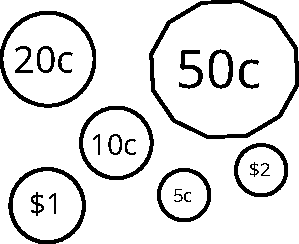
\includegraphics[width=\textwidth]{fig/42_coins}
\end{marginfigure}

Answer: The granny gave her grandson
\dotfill\medskip\par\mbox{}\dotfill\medskip\par\mbox{}\dotfill\bigskip.

\item The grandson buys a packet of Darrell Lea licorice for \$3.50.
How much does he have left over?

\medskip Number sentence:  \dotfill\medskip

Answer: The grandson has
\dotfill\medskip\par\mbox{}\dotfill\medskip
left over.

\item Professor Bumble created seven thousand and sixty-four robotic squirrels. If one thousand, two hundred and thirty-two of them ran away to join a nut-collecting competition, how many robotic squirrels are left with Professor Bumble?
% \marginnote{
% \large
% \opadd[operandstyle=\hole,
% resultstyle=\hole]{3427}{2051}}

\medskip Number sentence: \dotfill\medskip

Answer: Professor Bumble has \dotfill\medskip\par\mbox{}\dotfill\medskip\par\mbox{}\dotfill\bigskip
robotic squirrels left.

\item Princess Fluffybutt collected two thousand and one sparkly unicorn horns. Later, she found another seven thousand, nine hundred and ninety-eight horns while searching in her royal garden. How many sparkly unicorn horns does Princess Fluffybutt have now?

\medskip Number sentence: \dotfill\medskip

Answer: Princess Fluffybutt has 
\dotfill\medskip\par\mbox{}\dotfill\medskip\par\mbox{}\dotfill\bigskip
sparkly unicorn horns.

\end{enumerate}

\clearpage\section{Problem set \textnumero 43}

\begin{enumerate}
\item \marginnote{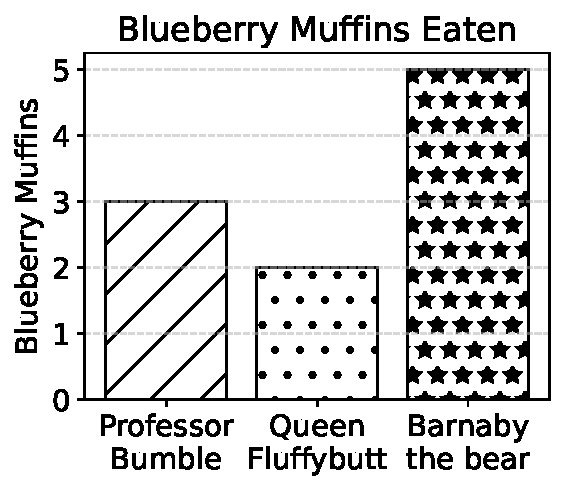
\includegraphics[width=0.5\textwidth]{fig/43_muffins.pdf}}
Princess Fluffybutt held a high tea for her birthday at Fluffybutt Manor.
The graph on the right shows how many blueberry muffins each guest ate.
Who ate the most?

Answer: \dotfill\medskip\par
ate the most with \dotfill blueberry muffins.

\item Princess Penelope collected two thousand four hundred and eighty-two rainbow-colored bouncy balls. A mischievous dragon stole one thousand and thirty-one of them. How many bouncy balls does Princess Penelope have left?
% \marginnote{
% \large
% \opadd[operandstyle=\hole,
% resultstyle=\hole]{3427}{2051}}

\medskip Number sentence: \dotfill\medskip

Answer: Princess Penelope has \dotfill\medskip\par\mbox{}\dotfill\medskip\par\mbox{}\dotfill\bigskip
bouncy balls left.

\item Farmer Giles had one thousand and forty-three singing carrots in his garden. He planted two thousand three hundred and fifty-six more singing carrots. How many singing carrots does Farmer Giles have in total?

\medskip Number sentence: \dotfill\medskip

Answer: Farmer Giles has a total of
\dotfill\medskip\par\mbox{}\dotfill\medskip\par\mbox{}\dotfill\bigskip
singing carrots.

\item Professor Bumble invented three thousand nine hundred and sixty-four self-folding socks. His cat, Mr. Snuggles, ate one thousand two hundred and fifty-two of them. How many self-folding socks are left?

\medskip Number sentence: \dotfill\medskip

Answer: There are 
\dotfill\medskip\par\mbox{}\dotfill\medskip\par\mbox{}\dotfill\bigskip
self-folding socks left.

\end{enumerate}

\clearpage\section{Problem set \textnumero 44}

\begin{enumerate}
\item \marginnote{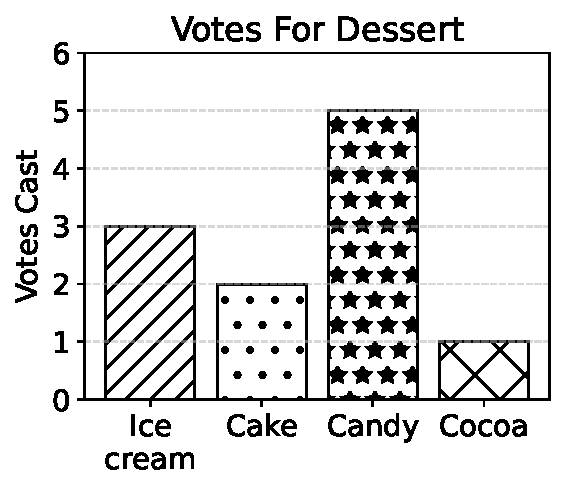
\includegraphics[width=0.5\textwidth]{fig/44_votes.pdf}}
Some hungry lads voted to decide what they would have for dessert.
How many boys were there in total? \medskip

Number sentence: \dotfill\medskip\par
There were \dotfill\medskip boys.

They ate \dotfill\medskip for dessert.

\item A flock of seven hundred and twenty-three rubber chickens crossed the road. One hundred and twelve were hit by a rogue shopping trolley. How many rubber chickens made it safely to the other side?\medskip

\medskip Number sentence: \dotfill\medskip

Answer: \dotfill\medskip\par\mbox{}\dotfill\medskip\par\mbox{}\dotfill\bigskip
rubber chickens made it safely to the other side.

\item Princess Fluffybutt had two thousand and thirty-one unicorn stickers. She gave one thousand and eleven to her pet aardvark, Bartholomew. How many unicorn stickers does Princess Fluffybutt have left?

\medskip Number sentence: \dotfill\medskip

Answer: Princess Fluffybutt has
\dotfill\medskip\par\mbox{}\dotfill\medskip\par\mbox{}\dotfill\bigskip
unicorn stickers left.

\item Professor Bumble had two boxes of disappearing ink pots. He wanted to know how many
ink pots he had in total, and worked the answer out using addition on the right.
Sadly, some of his working out disappeared! How many ink pots were in each box?\medskip\par
\marginnote{
\large
\begin{tabular}{ccc}
2 & \texttt{\_} & \quad{}\tabularnewline
\texttt{\_} & 7 & +\tabularnewline
\bottomrule
3 & 9 & \tabularnewline
\end{tabular}
}

\medskip Original number sentence: \dotfill\medskip

Answer: One box contained
\dotfill\medskip\par
ink pots, and the other \dotfill\medskip.

\end{enumerate}

\clearpage\section{Problem set \textnumero 45}

\begin{enumerate}
\item \marginnote{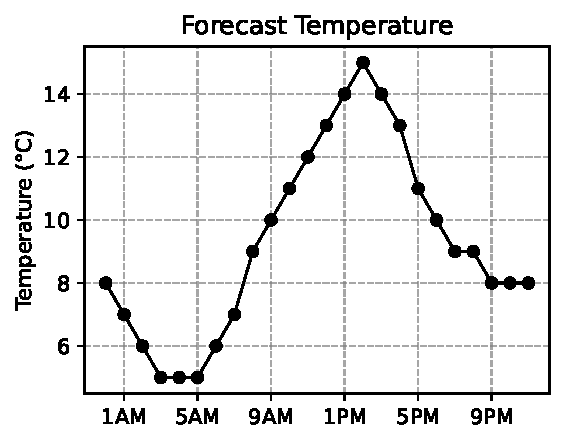
\includegraphics[width=0.5\textwidth]{fig/45_temp.pdf}}
The graph shows tomorrow's forecast temperature. What is the highest forecast temperature, and when?\medskip

It is expected to be \dotfill$^{\circ}$C\medskip\par
at \dotfill\medskip

\item Professor Snugglesworth had seven thousand, eight hundred and ninety-nine fluffy kittens. Three thousand, two hundred and thirty-four kittens decided to go on a trip to the moon. How many kittens were left with Professor Snugglesworth?

\medskip Number sentence:  \dotfill\medskip

Answer: 
\dotfill\medskip\par\mbox{}\dotfill\medskip
kittens remained.

\item \marginnote{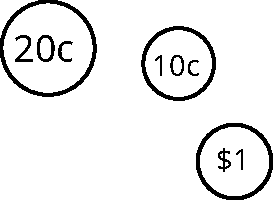
\includegraphics[width=0.5\textwidth]{fig/46_coins.pdf}}
A girl found the money shown on the right in her coat pocket. How much did she find?\medskip

Number sentence: \dotfill\medskip

The girl found \dotfill\medskip\par\mbox{}\dotfill.


\item A skateboarding unicorn collected two thousand and twenty-two rainbow-flavored lollipops. It then found another seven thousand, seven hundred and seventy-seven rainbow-flavored lollipops. How many rainbow-flavored lollipops does the skateboarding unicorn have altogether?

\medskip Number sentence:  \dotfill\medskip

Answer: The skateboarding unicorn has
\dotfill\medskip\par\mbox{}\dotfill\medskip\par\mbox{}\dotfill\bigskip
rainbow-flavored lollipops altogether.

\end{enumerate}


\clearpage\section{Problem set \textnumero 46}

\begin{enumerate}
  \item \marginnote{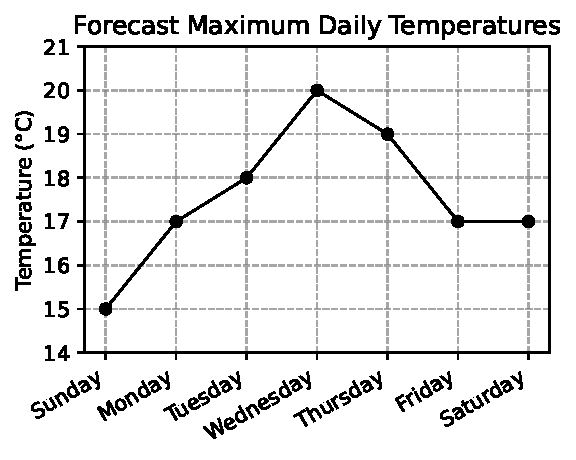
\includegraphics[width=0.5\textwidth]{fig/46_temp.pdf}}
  The graph shows daily forecast temperatures for the coming week.
  Which day has the warmest forecast temperature? What is it?\medskip
  
  It is expected to be \dotfill$^{\circ}$C\medskip\par
  on \dotfill\medskip.
  
\item
  Captain Calico started with nine thousand, nine hundred and
  ninety-nine rubber ducks in his bathtub. During a particularly bubbly
  bath, one thousand and one rubber ducks mysteriously vanished. How
  many rubber ducks remain in Captain Calico's
  bathtub?\medskip

  Number sentence:
  \dotfill\medskip\par

  Answer: There are
  \dotfill\medskip\par\mbox{}\dotfill\medskip\par\mbox{}\dotfill\bigskip
  rubber ducks remaining in Captain Calico's bathtub.

\item \marginnote{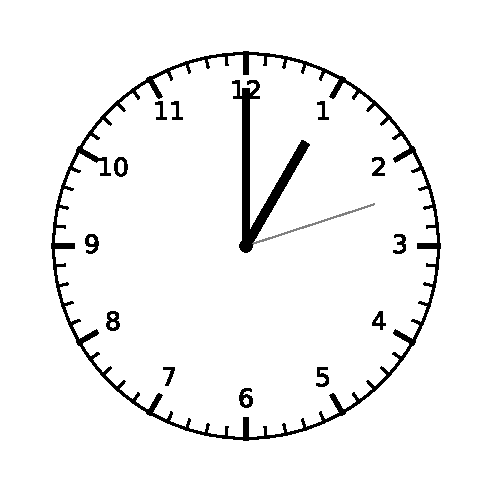
\includegraphics[width=0.5\textwidth]{fig/clock_0100.pdf}}
The clock shows the time in the afternoon. What time is it?\medskip

It is \dotfill\medskip.

\item A giraffe found three hundred and forty-five bouncy castles in a field. Later, it discovered another one hundred and twenty-two bouncy castles. How many bouncy castles did the giraffe find in total?

Number sentence: \dotfill\medskip

Answer: The giraffe found a total of
\dotfill\medskip\par\mbox{}\dotfill\medskip\par\mbox{}\dotfill\bigskip
bouncy castles.

\end{enumerate}



\clearpage\section{Problem set \textnumero 47}

\begin{enumerate}

\item \marginnote{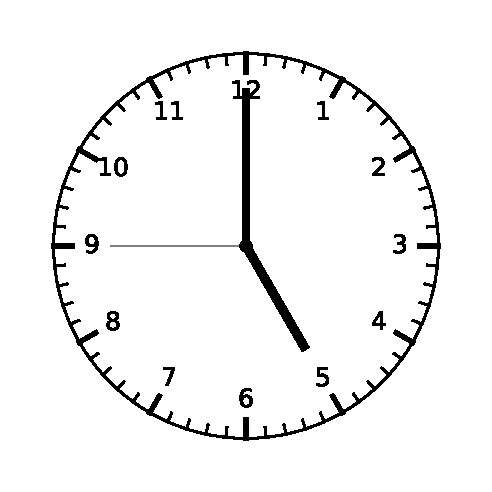
\includegraphics[width=0.5\textwidth]{fig/clock_0500.pdf}}
The clock shows the time in the afternoon. What time is it?\medskip

It is \dotfill\medskip.

\item
  A wizard had three hundred and twenty-seven rubber chickens. He
  accidentally turned one hundred and twelve of them into marshmallows.
  How many rubber chickens does he have left?\medskip

  Number sentence:
  \dotfill\medskip\par
  Answer: The wizard has
  \dotfill\medskip\par\mbox{}\dotfill\medskip\par\mbox{}\dotfill\bigskip
  rubber chickens left.

\item \marginnote{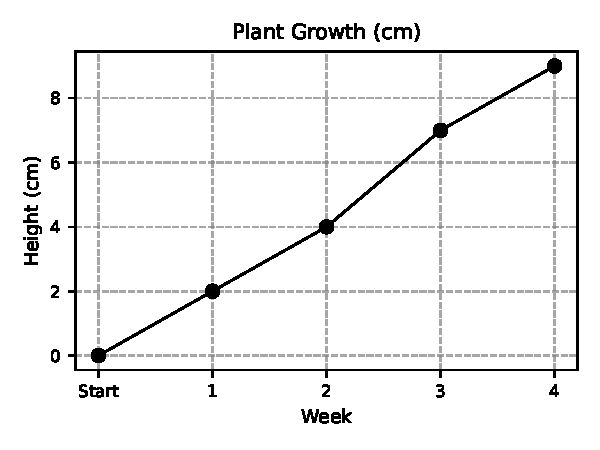
\includegraphics[width=0.5\textwidth]{fig/line_plant_growth}}
  Sally the Scientist is growing plants in her lab.
  The graph shows how the height of the plants changes over time.
  How tall was the plant after two weeks?\medskip

  The plant was \dotfill\medskip
  centimetres tall after two weeks.

\item
  Princess Penelope found two thousand, four hundred and fifty-six
  sparkly socks. A dragon gave her one thousand, three hundred and
  twenty-one more. How many sparkly socks does she have in total?\medskip\par
  Number sentence:
  \dotfill\medskip\par
  Answer: Princess Penelope has
  \dotfill\medskip\par\mbox{}\dotfill\medskip\par\mbox{}\dotfill\bigskip
  sparkly socks in total.

\end{enumerate}



\clearpage\section{Problem set \textnumero 48}

\begin{enumerate}

\item \marginnote{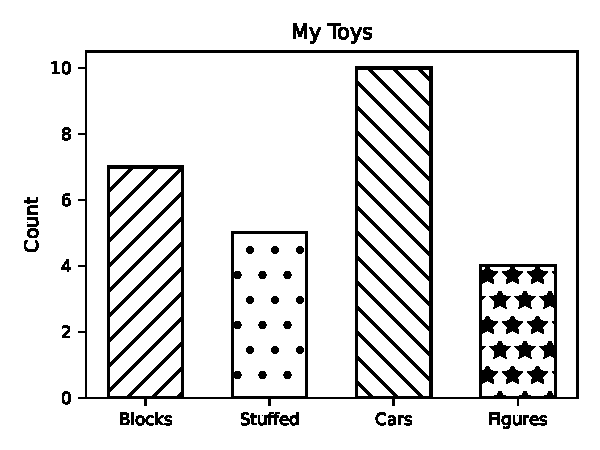
\includegraphics[width=0.5\textwidth]{fig/bar_my_toys.pdf}}
Gerry made a graph showing how many toys he has, broken down by type.
Which type of toy does he have the most of?\medskip

He has the most of \dotfill\medskip
toys.

\item How many toys does Gerry have in total?\medskip

Number sentence: \dotfill\medskip

Answer: Gerry has \dotfill\medskip
toys in total.

\item
  Professor Bumblebeard had seven hundred and twenty-three
  rainbow-flavored lollipops. A mischievous gnome stole one hundred and
  eleven of them. How many lollipops does Professor Bumblebeard have
  left?\medskip\par
  Number sentence:
  \dotfill\medskip\par
  Answer: Professor Bumblebeard has
  \dotfill\medskip\par\mbox{}\dotfill\medskip\par\mbox{}\dotfill\bigskip
  rainbow-flavored lollipops left.

\item \marginnote{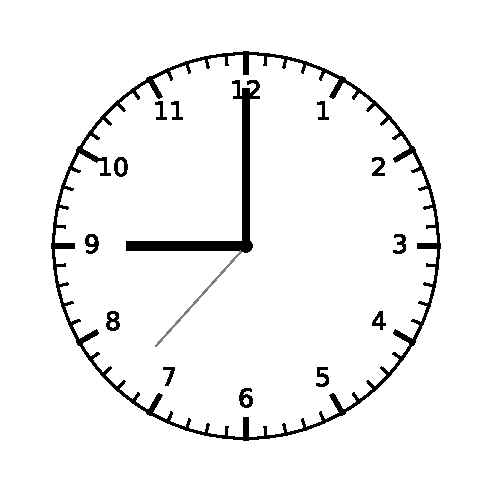
\includegraphics[width=0.5\textwidth]{fig/clock_0900.pdf}}
What's the time?\medskip

It is \dotfill\medskip.

\item
  A flock of four thousand and sixty-four fluffy, purple sheep were
  grazing in a field. Two thousand and thirty-one more fluffy, purple
  sheep joined them. How many fluffy, purple sheep are there in total?\medskip\par
  Number sentence:
  \dotfill\medskip\par
  Answer: There are
  \dotfill\medskip\par\mbox{}\dotfill\medskip\par\mbox{}\dotfill\bigskip
  fluffy, purple sheep in total.

\end{enumerate}


\clearpage\section{Problem set \textnumero 49}

\begin{enumerate}

\item \marginnote{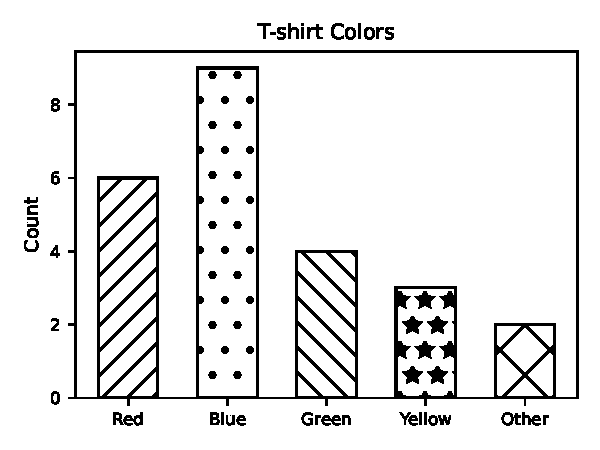
\includegraphics[width=0.5\textwidth]{fig/bar_tshirt_colors.pdf}}
A group of friends made a graph summarising the colours of their t-shirts.
How many friends are wearing red t-shirts?\medskip

There are \dotfill\medskip
friends wearing red t-shirts.

\item
  A wizard has two hundred and thirty-five rubber chickens. He
  accidentally turns one hundred and twelve of them into teacups. How
  many rubber chickens does the wizard have left?\medskip\par
  Number sentence:
  \dotfill\medskip\par
  Answer: The wizard has
  \dotfill\medskip\par\mbox{}\dotfill\medskip\par\mbox{}\dotfill\bigskip
  rubber chickens left.

\item \marginnote{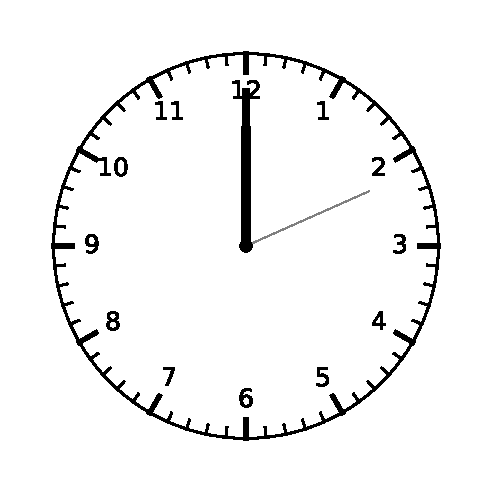
\includegraphics[width=0.5\textwidth]{fig/clock_1200.pdf}}
What's the time?\medskip

It is \dotfill\medskip.

\item
  Princess Penelope has one thousand, two hundred and forty-seven
  sparkly socks. A mischievous goblin gives her three thousand, one
  hundred and fifty-two more. How many sparkly socks does Princess
  Penelope have in total?\medskip\par
  Number sentence:
  \dotfill\medskip\par
  Answer: Princess Penelope has
  \dotfill\medskip\par\mbox{}\dotfill\medskip\par\mbox{}\dotfill\bigskip
  sparkly socks in total.

\item \marginnote{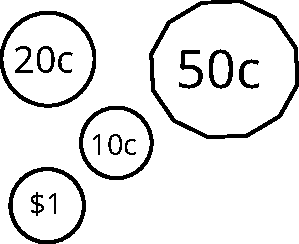
\includegraphics[width=0.5\textwidth]{fig/49_coins.pdf}}
How much money is there here?\medskip

Number sentence: \dotfill\medskip

There is \dotfill\medskip\par\mbox{}\dotfill\medskip\par\mbox{}\dotfill\bigskip.

\end{enumerate}



\clearpage\section{Problem set \textnumero 50}

\begin{enumerate}

\item \marginnote{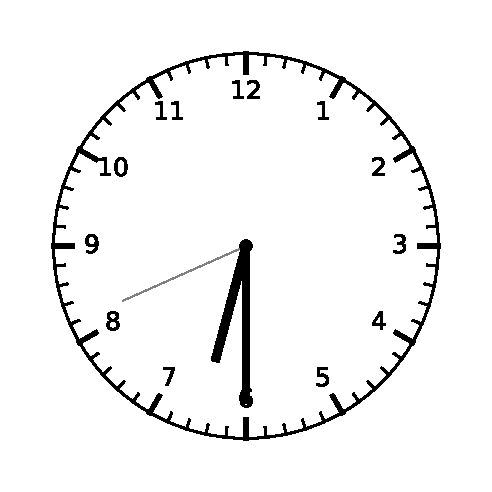
\includegraphics[width=0.5\textwidth]{fig/clock_0630.pdf}}
When Cole wakes up, his clock looks like this. What time does Cole wake up?\medskip

Cole wakes up at \dotfill\medskip.

\item
  Professor Bumblebeard collected three hundred and forty-seven shiny
  buttons. A mischievous gnome stole one hundred and twenty-three
  buttons to decorate his hat. How many buttons does Professor
  Bumblebeard have left?\medskip\par
  Number sentence:
  \dotfill\medskip\par
  Answer: Professor Bumblebeard has
  \dotfill\medskip\par\mbox{}\dotfill\medskip\par\mbox{}\dotfill\bigskip
  shiny buttons left.

\item \marginnote{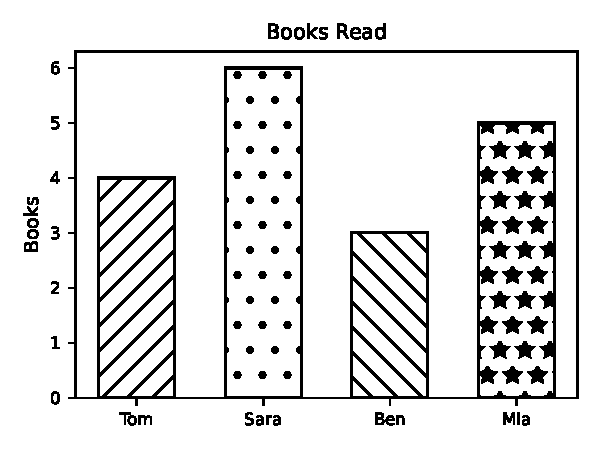
\includegraphics[width=0.5\textwidth]{fig/bar_books_read.pdf}}
Some children made a graph showing how many books they have read.
Who read more than 4 books?\medskip

\dotfill\medskip
read more than 4 books.

\item
  Princess Fluffybutt had nine thousand, eight hundred and seventy-six
  rainbow-colored lollipops. She ate five thousand, four hundred and
  thirty-two lollipops. How many lollipops does Princess Fluffybutt have
  left?\medskip\par
  Number sentence:
  \dotfill\medskip\par
  Answer: Princess Fluffybutt has
  \dotfill\medskip\par\mbox{}\dotfill\medskip\par\mbox{}\dotfill\bigskip
  lollipops left.

\end{enumerate}

\clearpage\section{Problem set \textnumero 51}

\begin{enumerate}
\item There are four clocks hanging on the wall. What time is it on each clock?\medskip\par
\begin{figure}[h]
  \centering
  \begin{tabular}{>{\centering}p{0.33\columnwidth}>{\centering}p{0.33\columnwidth}>{\centering}p{0.33\columnwidth}>{\centering}p{0.33\columnwidth}}
  Clock A & Clock B & Clock C & Clock D\tabularnewline
  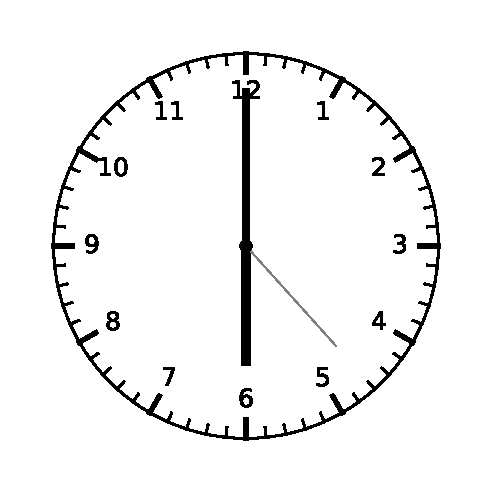
\includegraphics[width=0.33\columnwidth]{fig/clock_1800.pdf} & 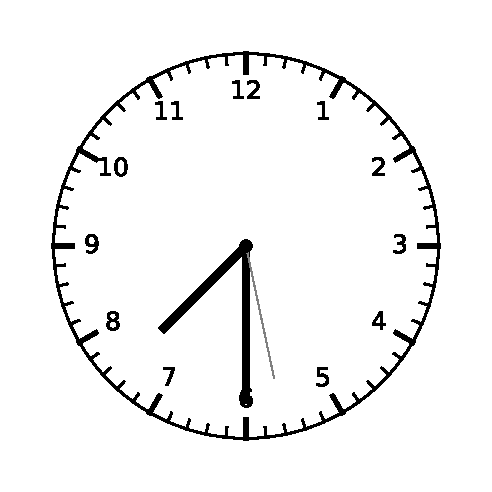
\includegraphics[width=0.33\columnwidth]{fig/clock_0730.pdf} & 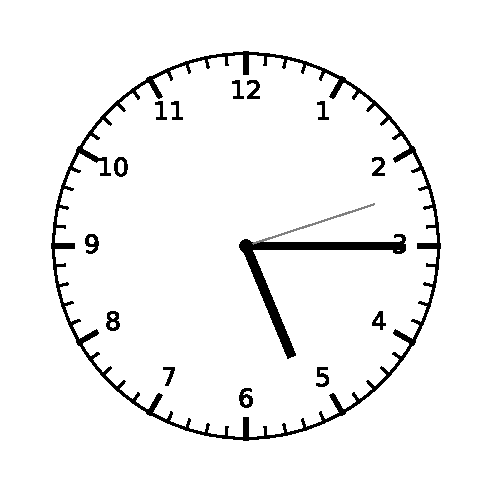
\includegraphics[width=0.33\columnwidth]{fig/clock_0515.pdf} & 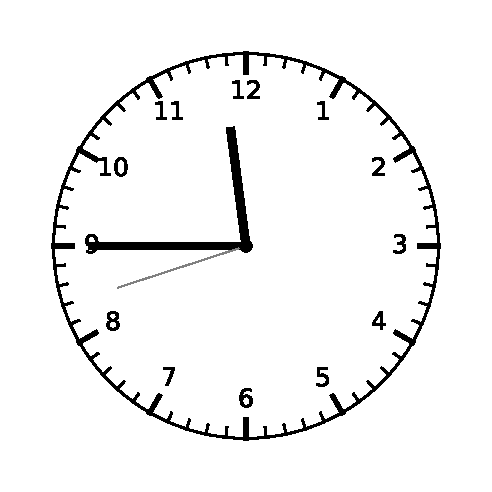
\includegraphics[width=0.33\columnwidth]{fig/clock_1145.pdf}\tabularnewline
  \end{tabular}
\end{figure}
Clock A shows \dotfill\medskip,\par
Clock B shows \dotfill\medskip,\par
Clock C shows \dotfill\medskip, and\par
Clock D shows \dotfill\medskip.

\item In the mystical land of Goblinia, a coffee costs one trillion kroner.
Gleem the goblin bought a coffee for himself and two for his mum. How much did he spend?\medskip\par
Answer: Gleem spent \dotfill\medskip\par\mbox{}\dotfill\medskip kroner.

\item \marginnote{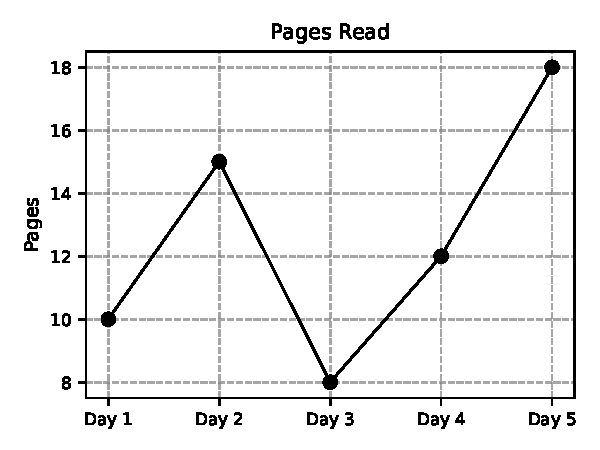
\includegraphics[width=0.5\textwidth]{fig/line_pages_read.pdf}}
Robert the rabbit made a graph showing how many pages he read each day.
How many pages did he read on day three?\medskip

Answer: Robert read \dotfill\medskip pages on day three.
\end{enumerate}

\clearpage\section{Problem set \textnumero 52}

\begin{enumerate}
\item \marginnote{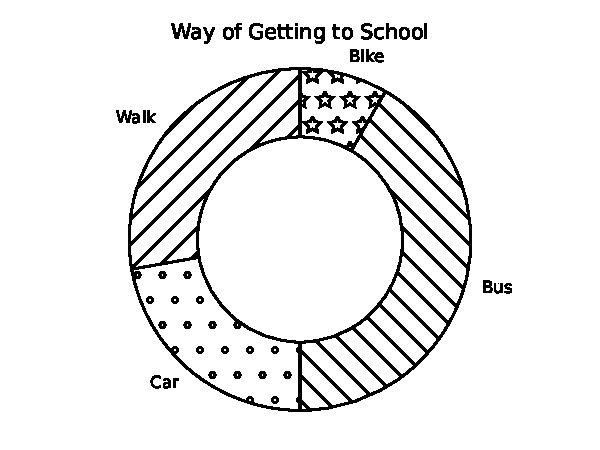
\includegraphics[width=0.5\textwidth]{fig/pie_to_school.pdf}}
The pie chart shows how students get to school. After the bus, what's the second most popular way?\medskip

The second most popular way to get to school is \dotfill\medskip\par\dotfill\medskip.

\item A giant purple penguin found three hundred and twenty-seven lost socks. He then found one hundred and fifty-two more. How many socks did the penguin find in total?\medskip\par
Number sentence: \dotfill\medskip\par
Answer: The giant purple penguin found 
\dotfill\medskip\par\mbox{}\dotfill\medskip\par\mbox{}\dotfill\bigskip
 socks in total.
\item \marginnote{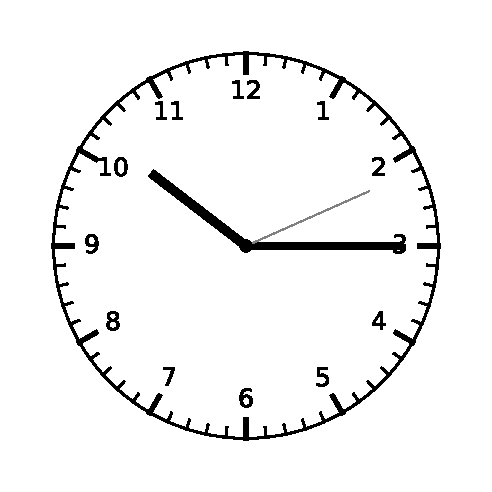
\includegraphics[width=0.5\textwidth]{fig/clock_1015.pdf}}
The time is \dotfill\medskip\par\dotfill\medskip.

\item Princess Fluffybutt had eight thousand, seven hundred and sixty-five rainbow-colored carrots. She ate two thousand, three hundred and forty-one of them. How many rainbow-colored carrots does she have left?\medskip\par
Number sentence: \dotfill\medskip\par
Answer: Princess Fluffybutt has 
\dotfill\medskip\par\mbox{}\dotfill\medskip\par\mbox{}\dotfill\bigskip
 rainbow-colored carrots left.
\end{enumerate}

\clearpage\section{Problem set \textnumero 53}

\begin{enumerate}
\item \marginnote{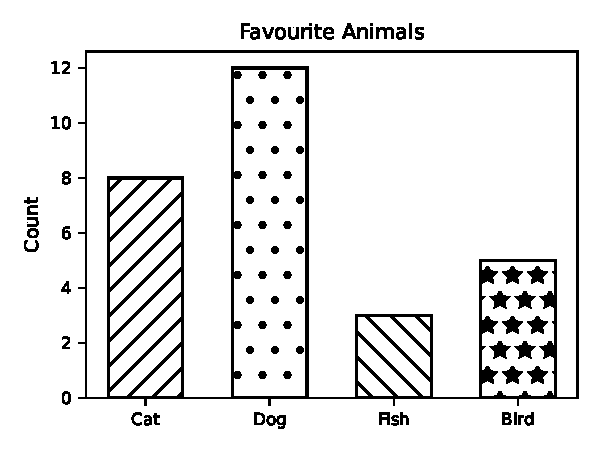
\includegraphics[width=0.5\textwidth]{fig/bar_fav_animals.pdf}}
A group of friends made a graph showing their favourite animals.
How many friends like dogs?\medskip

\dotfill\medskip friends like dogs.

\item A grumpy gargoyle found seven hundred and sixty-five shiny bottle caps. He then found two hundred and thirty-one more. How many bottle caps does the gargoyle have in total?\medskip\par
Number sentence: \dotfill\medskip\par
Answer: The gargoyle has 
\dotfill\medskip\par\mbox{}\dotfill\medskip\par\mbox{}\dotfill\bigskip
 bottle caps in total.
\item Princess Penelope had three thousand and forty-two rainbow-colored lollipops. She ate one thousand and twenty of them. How many lollipops does she have left?\medskip\par
Number sentence: \dotfill\medskip\par
Answer: Princess Penelope has 
\dotfill\medskip\par\mbox{}\dotfill\medskip\par\mbox{}\dotfill\bigskip
 lollipops left.

\item \marginnote{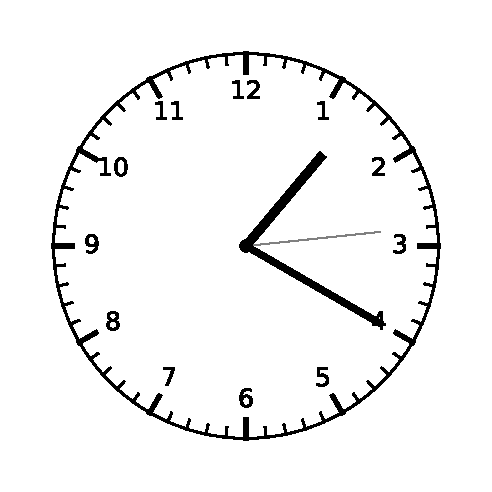
\includegraphics[width=0.5\textwidth]{fig/clock_0120.pdf}}
The time is \dotfill\medskip\par\dotfill\medskip.

\end{enumerate}

\clearpage\section{Problem set \textnumero 54}

\begin{enumerate}
\item \marginnote{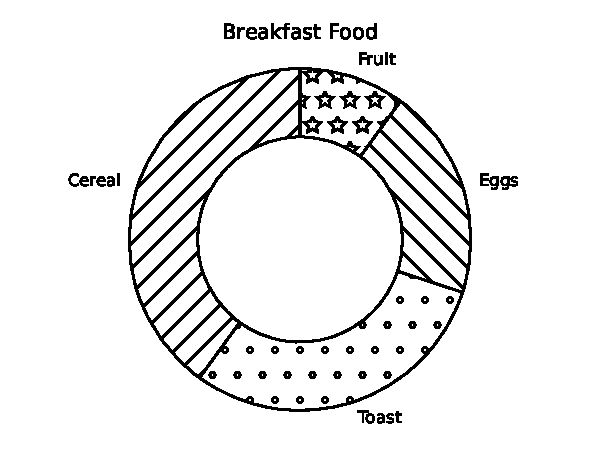
\includegraphics[width=0.5\textwidth]{fig/pie_breakfast_food.pdf}}
The pie chart shows what students eat for breakfast.
Which food is the most popular?\medskip

The most popular food is \dotfill\medskip.

 \item Write the time for each clock. Use digital time, like "5:00" or "5:30".\medskip

 \begin{figure}[h]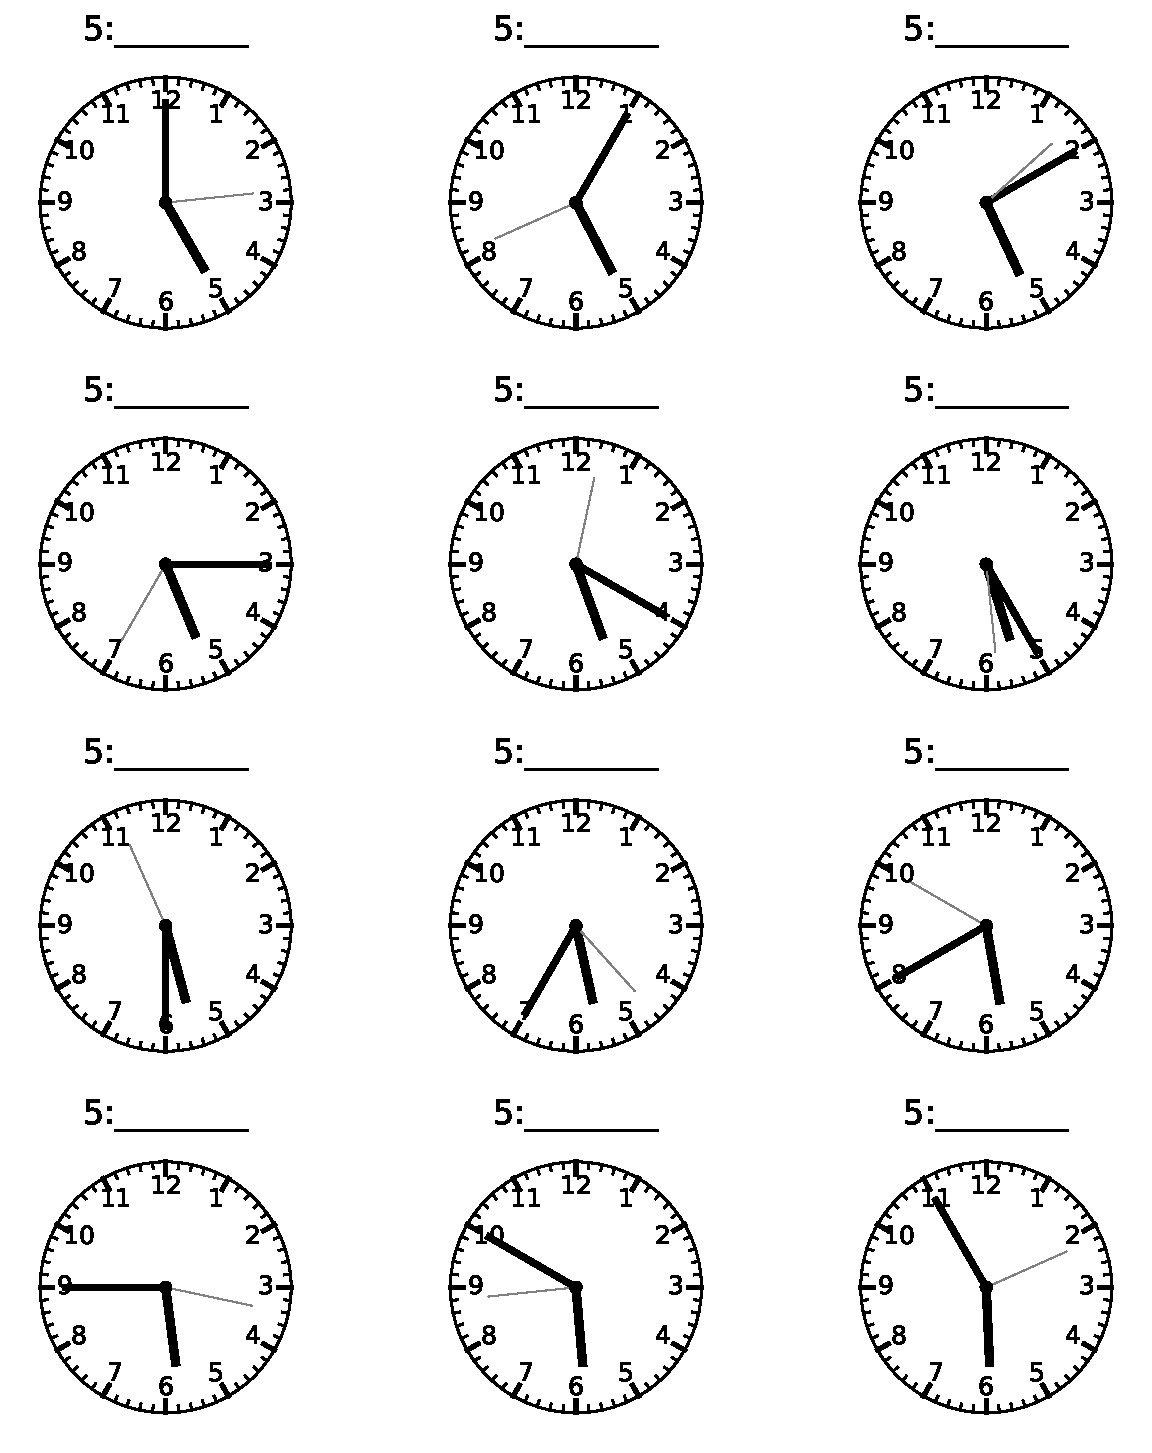
\includegraphics[width=\textwidth]{fig/clock_grid_0500.pdf}\end{figure}

\item A library costs one million dollars to build. A bridge costs one billion dollars. Which one is more expensive?\medskip\par
The \dotfill\medskip is more expensive.

\end{enumerate}

\clearpage\section{Problem set \textnumero 55}

\begin{enumerate}
\item A flock of two hundred and thirty-five singing sausages flew into Professor Bumble's garden. One hundred and twelve sausages decided to stay for tea. How many sausages flew away?\medskip\par
Number sentence: \dotfill\medskip\par
Answer: 
\dotfill\medskip\par\mbox{}\dotfill\medskip\par\mbox{}\dotfill\bigskip
 sausages flew away.

\item The graph shows 85 years of average maximum monthly temperatures at Sydney Airport, for the months of January and June.
\begin{figure}[h]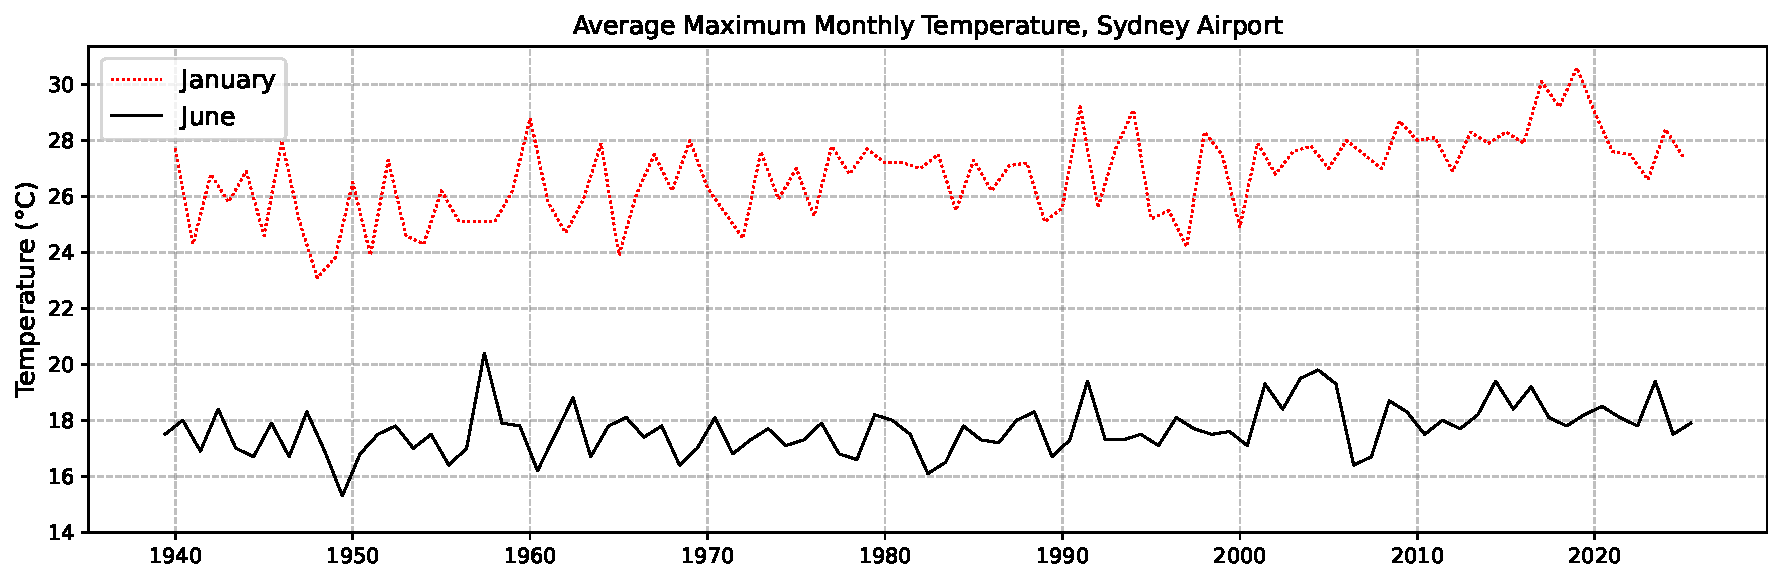
\includegraphics[width=1.5\textwidth]{fig/line_max_monthly_temp_syd.pdf}\end{figure}

Which month is hotter, on average?\medskip\dotfill\par
Why? \dotfill\medskip\par\mbox{}\dotfill\medskip\par\mbox{}\dotfill\bigskip

\item Princess Penelope collected four thousand, five hundred and sixty-seven sparkly stickers. She gave two thousand, three hundred and twenty-one stickers to her pet dragon, Sparky. How many stickers does Princess Penelope have left?\medskip\par
Number sentence: \dotfill\medskip\par
Answer: Princess Penelope has 
\dotfill\medskip\par\mbox{}\dotfill\medskip\par\mbox{}\dotfill\bigskip
 stickers left.

\end{enumerate}

\clearpage\section{Problem set \textnumero 56}

\begin{enumerate}

\item \marginnote{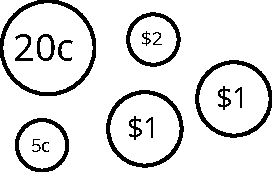
\includegraphics[width=0.5\textwidth]{fig/56_coins.pdf}}
How much money is there in total?\medskip

Number sentence: \dotfill\medskip

The total is \dotfill\medskip\par\mbox{}\dotfill\medskip.\par

\item The graph shows 81 years of average maximum monthly temperatures at Seattle-Tacoma Airport, for the months of January and June.
\begin{figure}[h]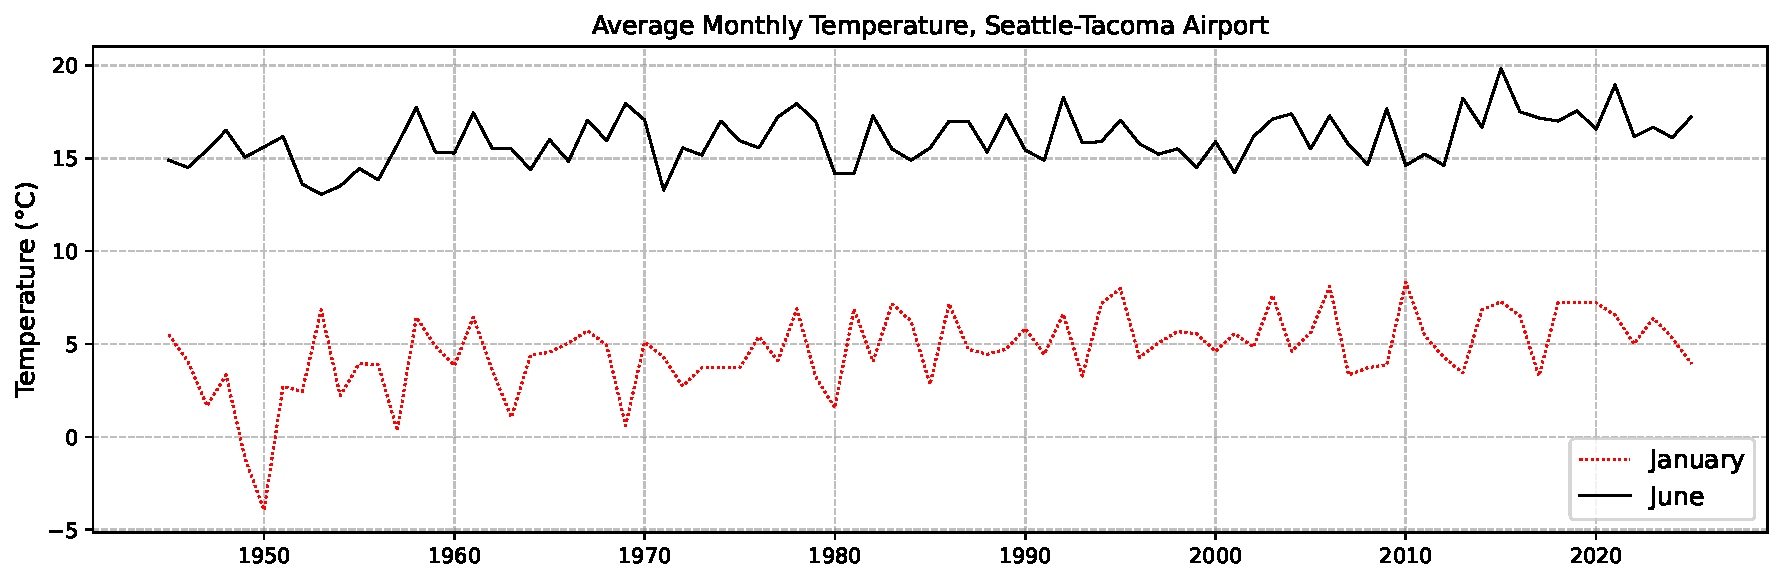
\includegraphics[width=1.5\textwidth]{fig/line_monthly_temp_sea.pdf}\end{figure}

Which month is hotter, on average?\medskip\dotfill\par
Why? \dotfill\medskip\par\mbox{}\dotfill\medskip\par\mbox{}\dotfill\bigskip\par
Compare your answer with yesterday's answer. \dotfill\medskip\par\mbox{}\dotfill\medskip\par\mbox{}\dotfill\bigskip


\item \marginnote{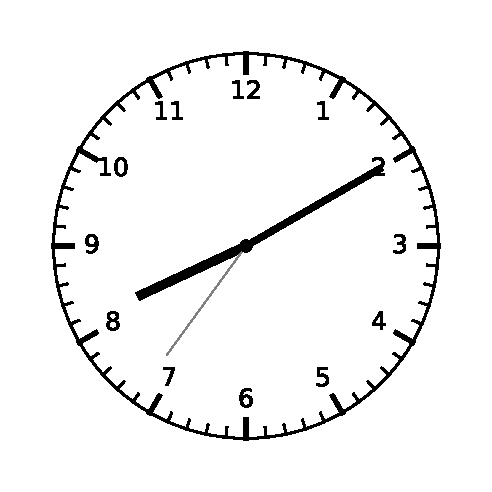
\includegraphics[width=0.5\textwidth]{fig/clock_0810.pdf}}
 It is \_\_\_ : \_\_\_\_\_\_ . \bigskip\par
 The time is \dotfill past \dotfill\medskip.
 
\item All the balls in the big box are blue. I reach into the box and pull out a red ball. Did I pull the ball from the big box?\medskip\par
Answer: \dotfill\medskip
\end{enumerate}

\clearpage\section{Problem set \textnumero 57}

\begin{enumerate}
\item There are some oranges in the fruit bowl. My dad asks me to pick an apple from the fruit bowl. Is this possible?\medskip\par
Answer: \dotfill\medskip

\item \marginnote{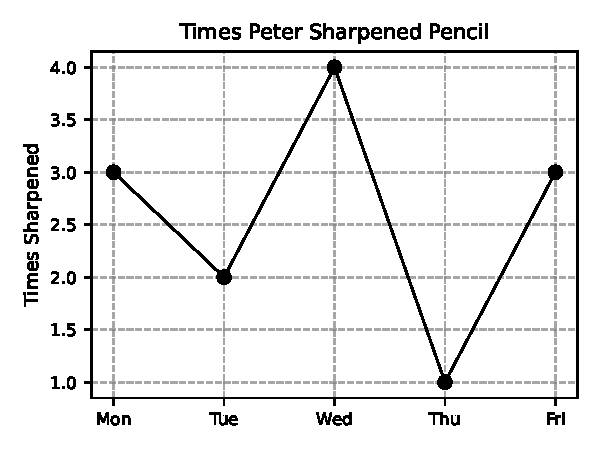
\includegraphics[width=0.5\textwidth]{fig/line_pencil_sharpenings.pdf}}
How many times did Peter sharpen his pencil on Tuesday?\bigskip\par
Answer: Peter sharpened his pencil \dotfill\bigskip times on Tuesday.

\item A wizard has two hundred and thirty-five rubber chickens. He accidentally turns one hundred and eighteen of them into teacups. How many rubber chickens does the wizard have left?\medskip\par
Number sentence: \dotfill\medskip\par
Answer: The wizard has 
\dotfill\medskip\par\mbox{}\dotfill\medskip\par\mbox{}\dotfill\bigskip
 rubber chickens left.

\item \marginnote{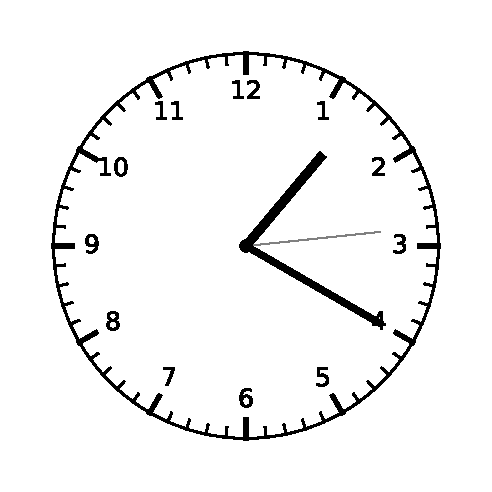
\includegraphics[width=0.5\textwidth]{fig/clock_0120.pdf}}
The time is \dotfill past \dotfill\bigskip.\par
It is \_\_\_ : \_\_\_\_\_\_ . \bigskip\par

\end{enumerate}

\clearpage\section{Problem set \textnumero 58}

\begin{enumerate}

\item Every cookie in the jar has chocolate chips. Dad gave me a cookie he said he got from the jar, and it doesn't have chocolate chips.
Did Dad make a mistake about where he got the cookie?\medskip\par
Answer: \dotfill\medskip

\item \marginnote{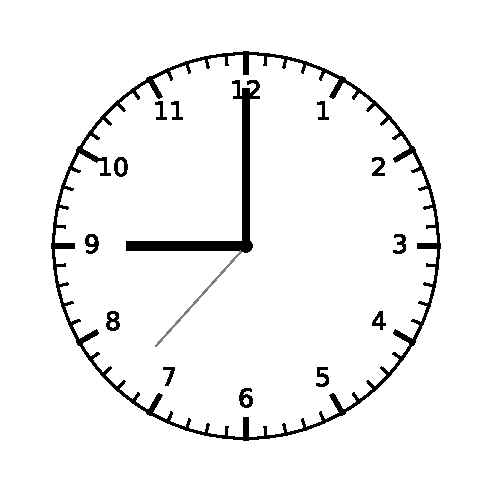
\includegraphics[width=0.5\textwidth]{fig/clock_0900.pdf}}
The time is \dotfill\medskip\par\dotfill\medskip.\par
It is \_\_\_ : \_\_\_\_\_\_ . \bigskip\par

\item A dancing pineapple had two hundred and forty-seven sparkly shoes. It lost one hundred and eighteen shoes during a conga line. How many shoes does the pineapple have left?\medskip\par
Number sentence: \dotfill\medskip\par
Answer: The dancing pineapple has 
\dotfill\medskip\par\mbox{}\dotfill\medskip\par\mbox{}\dotfill\bigskip
 sparkly shoes left.

\item \marginnote{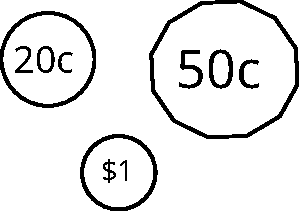
\includegraphics[width=0.5\textwidth]{fig/58_coins.pdf}}
How much money is there in total?\medskip

Number sentence: \dotfill\medskip

The total is \dotfill\medskip\par\mbox{}\dotfill\medskip.\par

\end{enumerate}

\clearpage\section{Problem set \textnumero 59}

\begin{enumerate}

\item All the pencils in my backpack are blue. Some of the things in my backpack are books. Can I have a red pencil in my backpack?\medskip\par
Answer: \dotfill\medskip

\item \marginnote{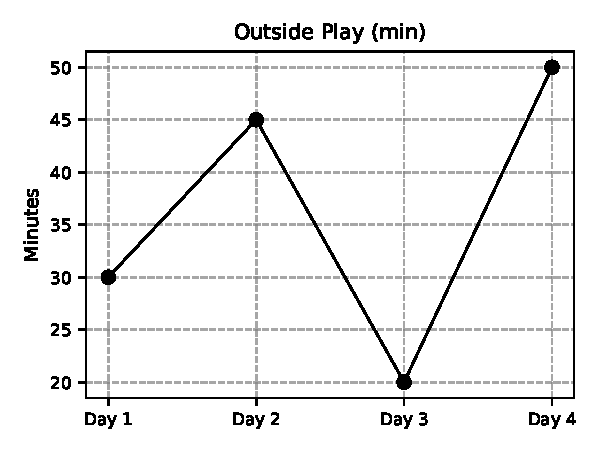
\includegraphics[width=0.5\textwidth]{fig/line_outside_play.pdf}}
On which days did the children play outside for more than half an hour?\bigskip\par
The children played outside for more than half an hour on \dotfill\bigskip\par\dotfill\bigskip.

\item Sir Reginald found one thousand and six lost socks. He then discovered seven hundred and ninety-nine more socks in his garden. 
How many socks did Sir Reginald find altogether?\medskip\par
Number sentence: \dotfill\medskip\par
Answer: Sir Reginald found 
\dotfill\medskip\par\mbox{}\dotfill\medskip\par\mbox{}\dotfill\bigskip
 socks altogether.

\item The graph shows monthly total retail sales (money spent in shops) in Australia.
In which month do people spend the most each year?\bigskip\par
\dotfill\bigskip\par
\begin{figure}[h]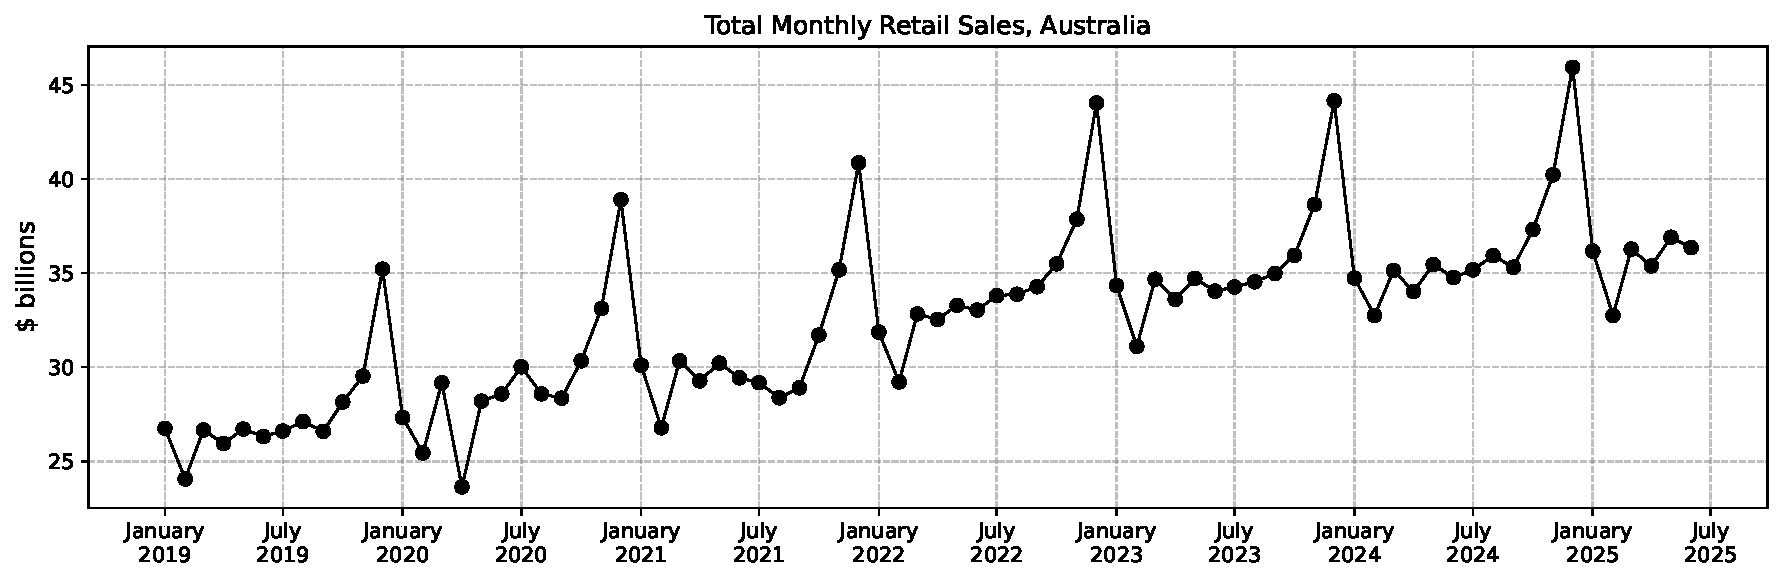
\includegraphics[width=1.3\textwidth]{fig/line_retail_sales.pdf}\end{figure}
Why do you think this is?
\dotfill\bigskip\par
\dotfill\bigskip\par

\end{enumerate}

\clearpage\section{Problem set \textnumero 60}

\begin{enumerate}

\item Some of the Lego blocks in the box are red. Every red block is a square. Can I find a round red block in the box?\medskip\par
Answer: \dotfill\medskip

\item \marginnote{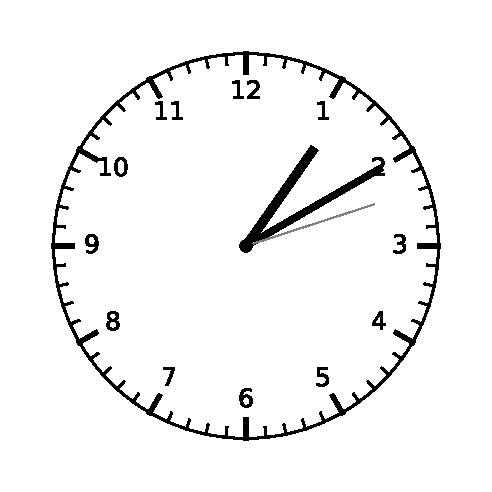
\includegraphics[width=0.5\textwidth]{fig/clock_0110.pdf}}
The time is \dotfill\medskip\par\dotfill\medskip.

\item Farmer Giles had five thousand, six hundred and seventy-eight singing carrots. A hungry badger ate three thousand, seven hundred and fifty-nine of them. How many singing carrots does Farmer Giles have now?\medskip\par
Number sentence: \dotfill\medskip\par
Answer: Farmer Giles now has 
\dotfill\medskip\par\mbox{}\dotfill\medskip\par\mbox{}\dotfill\bigskip
 singing carrots.

\item The graph shows the monthly retail sales of food retailing and cafes, restaurants and takeaway food.
How much was spent on cafes, restaurants, and takeaway food in the month you were born?\par
\begin{figure}[h]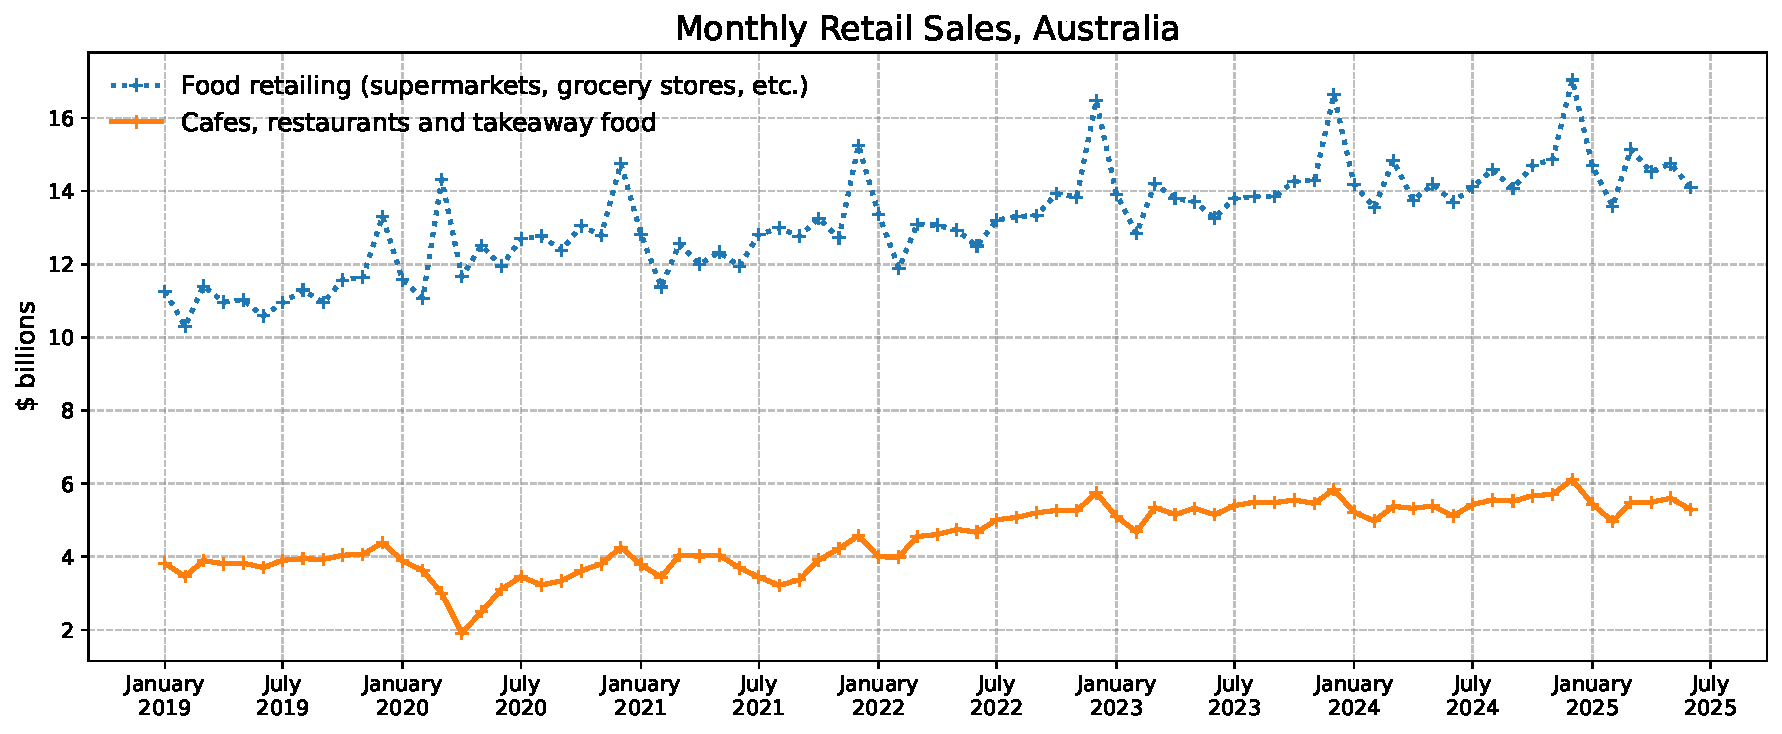
\includegraphics[width=1.3\textwidth]{fig/line_retail_sales_food.pdf}\end{figure}
People spent \dotfill\bigskip \par dollars in
the month of \dotfill\bigskip.

\end{enumerate}

\clearpage\section{Problem set \textnumero 61}

\begin{enumerate}

\item Professor Bumble created three hundred and sixty-two singing pineapples.
He then invented two thousand and fifty-seven more singing pineapples.
How many singing pineapples does Professor Bumble have in total?\bigskip\par
Number sentence: \dotfill\bigskip\par
Answer: Professor Bumble has a total of 
\dotfill\medskip\par\mbox{}\dotfill\medskip\par\mbox{}\dotfill\bigskip
  singing pineapples.

\item \marginnote{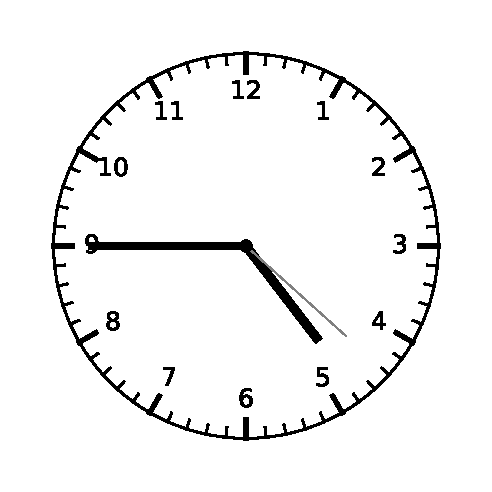
\includegraphics[width=0.5\textwidth]{fig/clock_0445.pdf}}
The time is \dotfill\bigskip\par\dotfill\bigskip.

\item Mum has ten marbles. Six are green. Could she have three red marbles?\bigskip\par
Answer: \dotfill\bigskip

\item About how many students were enrolled at Pascoe Vale Primary School in 2020?\bigskip\par
\begin{figure}[h]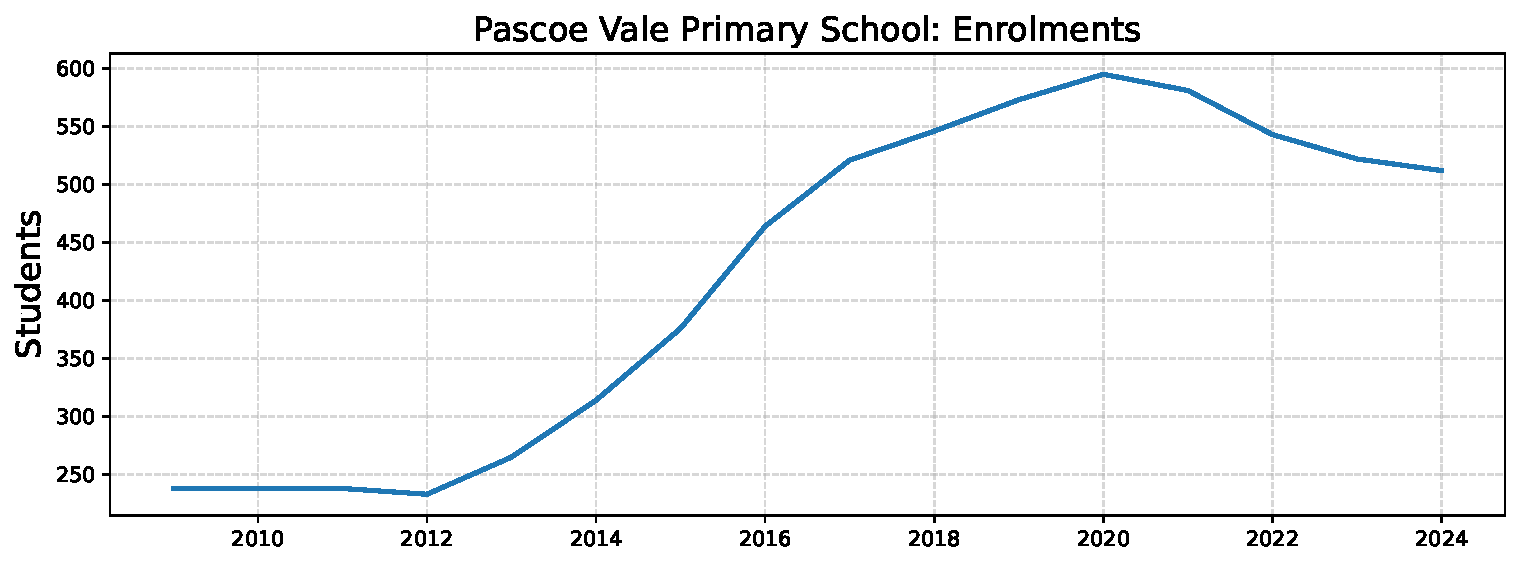
\includegraphics[width=1.3\textwidth]{fig/pvps_enrolments.pdf}\end{figure}
Answer: \dotfill\bigskip\par\dotfill\bigskip
\end{enumerate}

\clearpage\section{Problem set \textnumero 62}

\begin{enumerate}

\item \marginnote{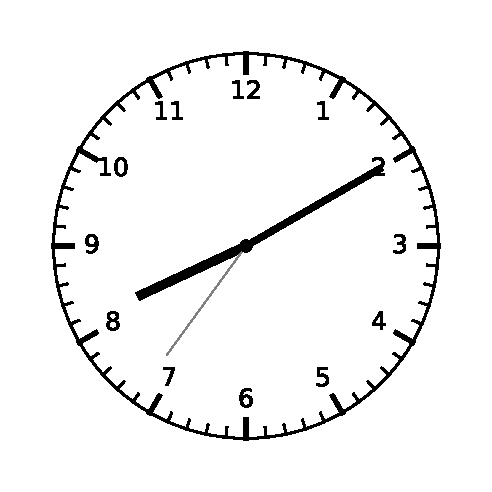
\includegraphics[width=0.5\textwidth]{fig/clock_0810.pdf}}
  The time is \dotfill\bigskip\par\dotfill\bigskip.
  
\item Queen Fluffybutt had nine hundred and ninety-one sparkly cupcakes. She ate six hundred and eighty-four of them. How many cupcakes does she have left?\medskip\par
Number sentence: \dotfill\medskip\par
Answer: Queen Fluffybutt has 
\dotfill\medskip\par\mbox{}\dotfill\medskip\par\mbox{}\dotfill\bigskip
 cupcakes left.

\item In the past few years, has the number of Grade 1/2 students at Pascoe Vale Primary School been increasing or decreasing?\bigskip\par
  \begin{figure}[h]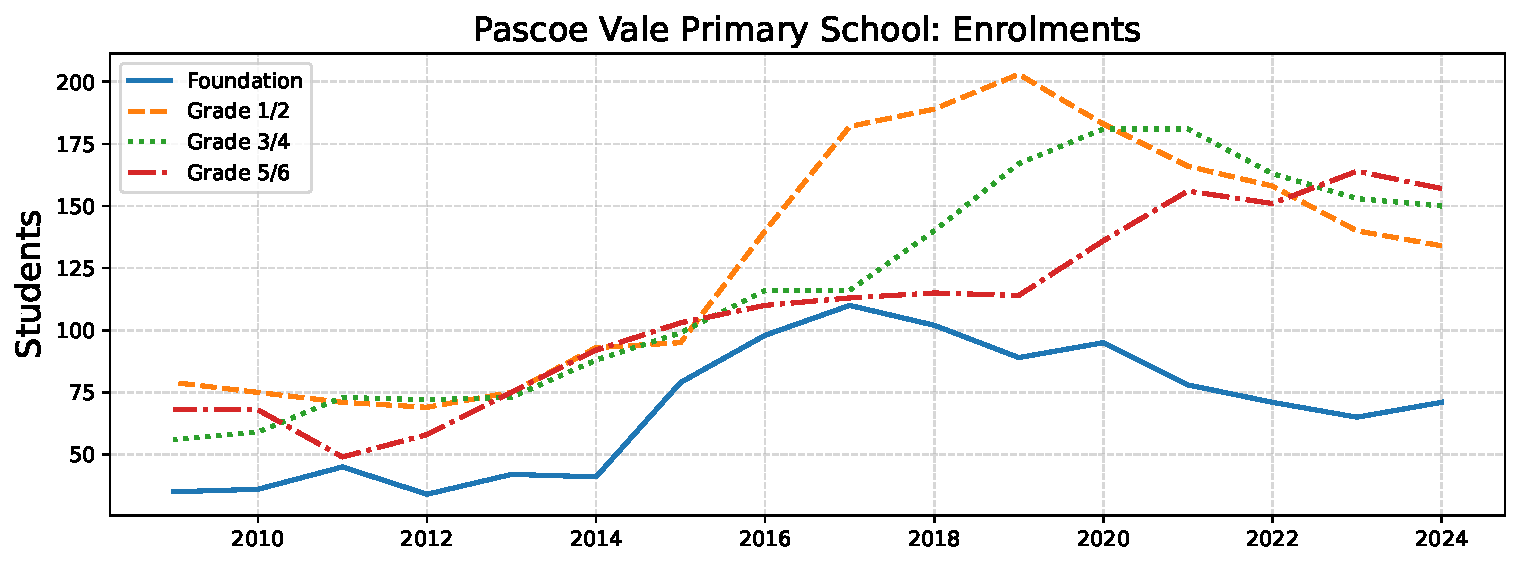
\includegraphics[width=1.3\textwidth]{fig/pvps_enrolments_grade.pdf}\end{figure}
  Answer: \dotfill\bigskip\par

\item Most PVPS students wear a blue shirt, and the rest wear a dress.
Sarah is wearing a green shirt. Does she attend PVPS?\bigskip\par
Answer: \dotfill\bigskip

\end{enumerate}

\clearpage\section{Problem set \textnumero 63}

\begin{enumerate}

\item \marginnote{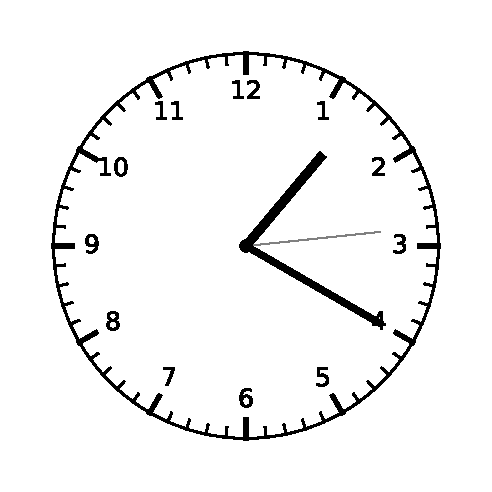
\includegraphics[width=0.5\textwidth]{fig/clock_0120.pdf}}
The time is \dotfill\bigskip\par\dotfill\bigskip.\par

\item Professor Bumble, the inventor, had nine thousand, nine hundred and thirty-nine cogs for his new invention.
He used nine thousand, three hundred and forty-five cogs. How many cogs does Professor Bumble have left?\bigskip\par
Number sentence: \dotfill\bigskip\par
Answer: Professor Bumble has 
\dotfill\bigskip\par\dotfill\bigskip cogs left.

\item Every kid on the playground is wearing a hat. Some of the kids are playing on the swings. If a kid is on the swings, is he wearing a hat?\bigskip\par
Answer: \dotfill\bigskip

\item Roughly how many kids were in the largest grade at PVPS in 2024?\bigskip\par
\marginnote{
\includegraphics[width=0.5\textwidth]{fig/pvps_enrolments_grade_2024.pdf}}

Answer: About \dotfill\bigskip students were in\par \dotfill\bigskip.\par

\end{enumerate}

\end{document}
